
\section{Experimental protocol}\label{app:proto}

\textbf{Models.} Qwen3-VL-2B-Instruct and Qwen2-VL-7B-Instruct (core pair), Qwen2.5-VL-7B-Instruct, Qwen3-VL-8B-Instruct
(36 layers), LLaVA-NeXT-7B and LLaVA-OneVision-7B (attention analyses only). \texttt{bfloat16}; eager attention
wherever hooks or a prune bias are required, SDPA otherwise. We note a ${\sim}2$ point kernel-dependent difference on
the 7B between the two implementations and always compare arms computed under the same kernel.

\textbf{Budgets.} Images are resized so that the processor's own \texttt{image\_grid\_thw} yields the target token
count ($\pm 8\%$); realised counts are recorded per arm and a contrast is voided if budgets drift by more than $10\%$.
Where pruning changes cost mid-network we report token-layers.

\textbf{Read-out.} The attention map is the final prompt token's attention over image-token columns, averaged over
heads \emph{before} normalising (the order matters: normalising per head first up-weights sink-heavy heads and shifts
the block-mean read-out by $11$ points on the 7B). The prompt must end at the answer-emission point; a prompt ending
elsewhere costs $36$--$42$ points on the arg-max read-out.

\textbf{Statistics.} Paired item bootstrap with 8000 resamples. Learned components use GroupKFold(5) grouped by item
$\times$ 3 seeds; the headline DWA result is additionally reproduced under a disjoint fold-seed set (difference
within $\pm1$ point). Run-to-run floor on coverage is $1$--$2.5$ points.

\textbf{Pipeline discipline.} An exactly $+0.0$ contrast with a $[+0.0,+0.0]$ interval is treated as a pipeline fault,
never a result; this rule caught a monkey-patch that silently failed to reach one model family. Every pruning run
asserts at runtime that the loaded model's attention module is the one that was patched.

\section{The DWA read-out: features, estimator, and the feature-block ablation}\label{app:feat_engine}

Let $a_i^{(\ell)}$ denote the head-mean attention at image cell $i$ and layer $\ell$, where
$i=1,\ldots,N$ and $\ell=0,\ldots,L-1$, read from the final prompt token over the image cells. We normalise
each map over the image cells,
\begin{equation}
    A_i^{(\ell)} = \frac{a_i^{(\ell)}}{\max\!\left(\sum_{j=1}^{N}a_j^{(\ell)},\epsilon\right)},
    \qquad \epsilon=10^{-12},
\end{equation}
where $j$ indexes image cells in the sum. Each cell is represented by its normalised depth profile,
$\bigl(\log(A_i^{(\ell)}+\epsilon)\bigr)_{\ell=0}^{L-1}$, so with $L=28$ each cell has $28$ features. The read-out
is a single closed-form ridge regression on these features,
\begin{equation}
    w = (X^\top X + \alpha I)^{-1} X^\top y, \qquad \alpha=1,
\end{equation}
with an unpenalised intercept, fitted out-of-fold (GroupKFold(5) $\times$ 3 group permutations, grouped by item)
to the coverage label $y_i$, the fraction of the ground-truth box inside the $W{=}0.25$ window centred at cell
$i$. Placement is the ring-masked arg-max of the score $s(c) = w_0 + \sum_{\ell=0}^{L-1} w_\ell \log A_\ell(c)$.

\textbf{The deployed vector.} The deployed read-out carries two further blocks,
$\mathbf{x}_i\in\mathbb{R}^{2L+7}$: (i) $L$ per-layer rank features,
$R_i^{(\ell)}=\mathrm{rank}_\downarrow\!\bigl(a_i^{(\ell)}\bigr)/(N-1)$, the cell's descending rank in layer
$\ell$'s map; and (ii) seven neighbourhood/geometry features --- the log $3\times3$ neighbourhood mean of the
read-out-band map (the band where attention first becomes question-conditioned,
$L_{\mathrm{lo}}=\mathrm{round}(0.57L)$ through $L-1$), the cell's horizontal and vertical coordinates, its
distance from the image centre, its distance to the nearest border, and two indicators for the last row and
column. Ranks are per-layer and item-relative; the geometry block is item-independent.

\textbf{Feature-block ablation.} Refitting the same estimator on \vstar\ ($191$ items) with feature blocks
removed, out-of-fold coverage of the $W{=}0.25$ window at the ring-masked arg-max:

\begin{table}[h]\centering\small
\caption{\textbf{The log-attention block carries the advantage.} Out-of-fold coverage on \vstar, by feature
block.}
\begin{tabular}{lcccc}
\toprule
model & block-mean read-out & log only ($L$) & log$+$rank ($2L$) & full ($2L{+}7$)\\
\midrule
Qwen3-VL-2B & $0.475$ & $0.638$ & $0.640$ & $\mathbf{0.655}$\\
Qwen2-VL-7B & $0.408$ & $0.574$ & $\mathbf{0.587}$ & $0.561$\\
\bottomrule
\end{tabular}\label{tab:featabl}
\end{table}

The log-attention block alone recovers $0.163$/$0.166$ of the block-mean gap --- $91\%$/$108\%$ of the full
vector's lift: the advantage is carried by the depth profile, and the rank/geometry blocks add $+0.017$ on
Qwen3 and $-0.013$ on Qwen2. They are kept in the deployed vector because they are free at fit time, but they
are not the mechanism; the main-text read-out quotes the log-attention score. Script:
\texttt{phase238\_feat\_ablation.py}.

\section{Intermediate metrics systematically over-report}\label{app:proxy}

Five times in this work an intermediate metric improved while end-task accuracy did not: a read-out that closed the
coverage gap but converted $3.1$ points worse; a ridge variant that tied on coverage and differed on the chosen cell
for two-thirds of items; an early-exit localiser free in coverage but $-3.7$ pooled at the end task; a
higher-resolution localiser that gained $+4.2$ coverage and $-3.7$ accuracy; and an objectness probe that retains the
evidence box far better than attention ($87\%$ vs.\ $72\%$) and converts to $-1.6$. We therefore report coverage only
as a diagnostic and gate every claim on end-task accuracy at matched compute.


\section{The transport measurement in full}\label{app:transport}

A forward pre-hook on every decoder layer adds $-10^4$ to the attention logits of chosen query rows over the
image-token columns, at chosen layers only. Masking \emph{all} text rows at \emph{all} layers destroys the answer
(KL $1.266$ / $0.532$, $42\%$ / $45\%$ of answers flip, $n{=}40$); masking only the answer token's row at all layers
does not (KL $0.025$, $3\%$ flip). Table~\ref{tab:prefix} localises the window.

\begin{table}[h]\centering\small
\caption{Prefix and suffix masks, all text rows, $n=40$ per model, V$^*$Bench at 300 tokens. The prefix mask
$L_0..\ell$ saturates at the full-mask value once $\ell$ passes the window; the suffix mask $L_\ell..\text{end}$
falls to zero once $\ell$ is past it. Both read the boundary at the same place, and the $36$-layer checkpoint puts
it at the same fraction of depth ($\ell{=}20$ of $36$).}
\begin{tabular}{lcccccc}
\toprule
& $\ell{=}4$ & $\ell{=}8$ & $\ell{=}12$ & $\ell{=}16$ & $\ell{=}20$ & $\ell{=}24$\\
\midrule
Qwen3 prefix $L_0..\ell$ (KL) & 0.082 & 0.549 & \textbf{1.278} & 1.259 & 1.215 & 1.257\\
Qwen3 suffix $L_\ell..$ (KL) & 0.967 & 0.880 & 0.320 & \textbf{0.014} & 0.002 & 0.001\\
Qwen3 suffix (answers flipped) & 53\% & 50\% & 20\% & 12\% & \textbf{0\%} & \textbf{0\%}\\
\midrule
Qwen2 prefix $L_0..\ell$ (KL) & 0.037 & 0.105 & 0.364 & \textbf{0.547} & 0.534 & 0.538\\
Qwen2 suffix $L_\ell..$ (KL) & 0.518 & 0.465 & 0.429 & \textbf{0.029} & 0.004 & 0.002\\
Qwen2 suffix (answers flipped) & 53\% & 47\% & 40\% & 5\% & 3\% & \textbf{0\%}\\
\midrule
Qwen3-8B (36L) prefix $L_0..\ell$ (KL) & 0.100 & 0.309 & 1.190 & \textbf{1.740} & 1.559 & 1.565\\
Qwen3-8B (36L) suffix $L_\ell..$ (KL) & 1.671 & 1.538 & 1.278 & 0.413 & \textbf{0.052} & 0.009\\
Qwen3-8B (36L) suffix (answers flipped) & 35\% & 45\% & 40\% & 15\% & 5\% & \textbf{0\%}\\
\bottomrule
\end{tabular}\label{tab:prefix}
\end{table}

\begin{figure}[h]\centering
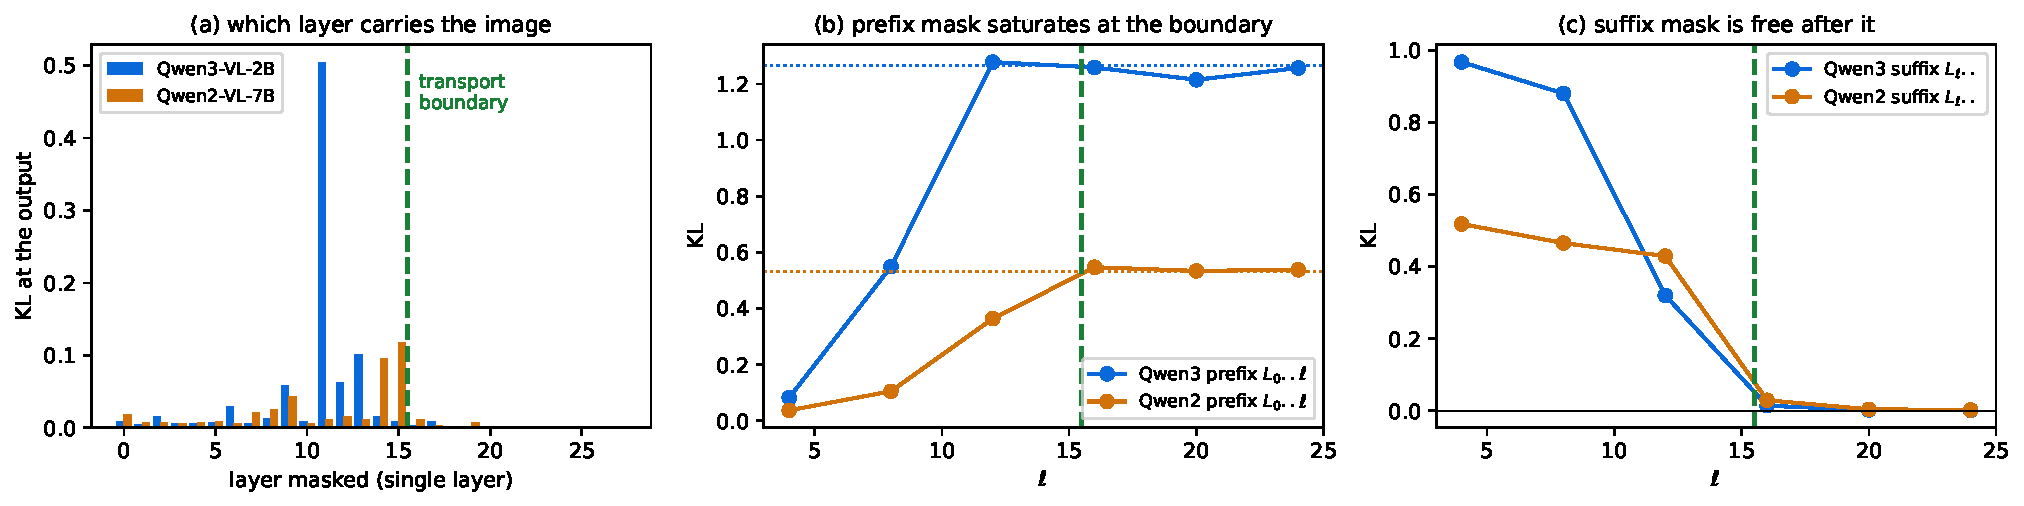
\includegraphics[width=\textwidth]{figs/fig_transport.pdf}
\caption{\textbf{The transport measurement.} (a) Masking one layer's image attention at a time: the effect is
concentrated well before the boundary and is at or below $0.0023$ from L20 on both models. (b) Masking a prefix
$L_0..\ell$ reaches the full-mask value (dotted) once $\ell$ passes the window. (c) Masking a suffix
$L_\ell..\text{end}$ costs nothing once $\ell$ is past it. Three readings, one boundary.}
\label{fig:transport}
\end{figure}

Single-layer masks peak at L11 on Qwen3 (KL $0.504$; next highest L13 at $0.101$) and at L15/L14 on Qwen2
($0.118$/$0.096$). From L20 onward every layer is at or below $0.0023$ on both models. On Qwen3-VL-8B, which has
$36$ layers, the same behaviour appears at L21, i.e.\ the same $0.57$ fraction of depth.

\paragraph{Three independent readings of the same boundary.} The masks are one. Pruning is the second: discarding
$90\%$ of visual tokens at the boundary costs $+0.0$ to $+0.5$ points across ten stratum-cells, whereas moving the
same cut to $\ell{=}4$ costs $5.2$ more on one model ($0.5$ on the other), and a taper that removes half the tokens
at $\ell{=}9$--$12$ loses $3.5$ points against not pruning at matched tokens while buying nothing over a single cut
($-1.0$). Read-out depth is the third: restricting the localiser to layers $\le$ L20 costs $-0.5$ and $+1.6$ points
of coverage, while restricting it to $\le$ L16 costs $9.4$ and $22.0$. Transport finishes at the boundary; the
signal the ranking reads is produced after it.

\section{Depth structure across checkpoints}\label{app:depth}

\begin{table}[h]\centering\small
\caption{Where each quantity falls, per checkpoint. The transport boundary and the read-out band are fractions of
depth, not fixed layer indices, which is what lets both policies transfer to a $36$-layer model unchanged. The
$36$-layer boundary is masked: its suffix is harmless at L20 and zero from L24, the same fractions as the pair.}
\begin{tabular}{lccccc}
\toprule
checkpoint & layers & block-mean band & read-out band & boundary & boundary / depth\\
\midrule
Qwen3-VL-2B & 28 & L16--L26 & L17--L20 & L16 & 0.57\\
Qwen2-VL-7B & 28 & L15--L26 & L19--L22 & L16 & 0.57\\
Qwen2.5-VL-7B & 28 & L16--L26 & --- & L16 & 0.57\\
Qwen3-VL-8B & \textbf{36} & L20--L33 & --- & \textbf{L21} & 0.57\\
\bottomrule
\end{tabular}\label{tab:depth}
\end{table}

\section{Full paired comparison against published rules}\label{app:paired}

\begin{table}[h]\centering\small
\caption{DWA minus each alternative on V$^*$Bench, paired on identical items, pooled over strata,
$n=191$ ($190$ for LASER, one item missing). All six published-rule contrasts clear zero on both models.
Bootstrap $95\%$ CIs, $8{,}000$ resamples, matching the protocol in Appendix~\ref{app:proto}.}
\begin{tabular}{lcc}
\toprule
contrast & Qwen3-VL-2B & Qwen2-VL-7B\\
\midrule
$-$ \texttt{uniform@600} (equal-compute bar) & \gd{$+8.9$ [$+0.5,+17.3$]}~\ok & \gd{$+12.0$ [$+4.7,+19.4$]}~\ok\\
$-$ fixed-layer crop (L14) & \gd{$+34.6$ [$+25.7,+43.5$]}~\ok & \gd{$+31.9$ [$+24.1,+39.8$]}~\ok\\
$-$ block-mean arg-max & \gd{$+10.5$ [$+4.2,+16.8$]}~\ok & \gd{$+11.0$ [$+4.7,+17.8$]}~\ok\\
$-$ LASER$^\dagger$ & \gd{$+7.9$ [$+1.1,+14.7$]}~\ok & \gd{$+8.9$ [$+3.1,+14.7$]}~\ok\\
\midrule
\multicolumn{3}{l}{\emph{controls, not baselines}}\\
$-$ gate-max & $+3.7$ [$-2.1,+9.4$] & \gd{$+9.4$ [$+3.7,+15.2$]}~\ok\\
$-$ gradient-boosted tree & $-0.5$ [$-4.7,+4.2$] & \gd{$+7.3$ [$+2.1,+13.1$]}~\ok\\
$-$ DWA refit, disjoint fold seeds & $-1.0$ [$-3.1,+1.0$] & $+1.0$ [$-1.0,+3.1$]\\
$-$ oracle placement & $-15.2$ [$-22.5,-8.4$]~\no & $-17.3$ [$-24.6,-9.9$]~\no\\
\bottomrule
\end{tabular}\label{tab:paired}
\end{table}

Taking these six together with the three pooled block-mean contrasts in Table~\ref{tab:hrpaired}, DWA
beats a published rule in nine of nine pooled comparisons. It does not beat the equal-compute bar everywhere, which
is a separate claim and the subject of the scope law. The fold-seed control matters most. Refitting DWA under three disjoint fold seeds moves the pooled result by
$1.0$ point or less on both models, so the margin is not an artefact of which items landed in which fold. The
oracle row is the remaining headroom: even the best rule we have is $15$--$17$ points below perfect placement.

\begin{table}[h]\centering\footnotesize
\setlength{\tabcolsep}{3pt}
\caption{HR-Bench, DWA minus each alternative, $n=400$ per stratum, $800$ per cell. DWA is transferred:
its weights were fit on V$^*$Bench and applied here with nothing refit. Placement quality replicates; the scope
law replicates with it.}
\begin{tabular}{llccc}
\toprule
& & HR-4K Qwen3-2B & HR-4K Qwen2-7B & HR-8K Qwen3-2B\\
\midrule
\multirow{3}{*}{vs.\ bar} & single & \gd{$+10.2$ [$+5.5,+15.0$]}~\ok & \gd{$+9.2$ [$+4.5,+14.2$]}~\ok & \gd{$+8.8$ [$+3.5,+13.8$]}~\ok\\
 & cross & $-8.8$ [$-14.0,-3.5$]~\no & $-6.0$ [$-11.5,-0.8$]~\no & $-8.8$ [$-14.5,-2.8$]~\no\\
 & pooled & $+0.8$ [$-2.8,+4.4$] & $+1.6$ [$-1.9,+5.2$] & $+0.0$ [$-3.9,+4.0$]\\
\midrule
\multirow{3}{*}{vs.\ block-mean} & single & \gd{$+7.8$ [$+4.0,+11.5$]}~\ok & \gd{$+15.0$ [$+10.2,+19.8$]}~\ok & \gd{$+5.2$ [$+1.2,+9.2$]}~\ok\\
 & cross & $+1.8$ [$-2.8,+6.2$] & \gd{$+16.8$ [$+12.0,+21.5$]}~\ok & $+2.2$ [$-2.5,+6.8$]\\
 & pooled & \gd{$+4.8$ [$+1.9,+7.6$]}~\ok & \gd{$+15.9$ [$+12.6,+19.2$]}~\ok & \gd{$+3.8$ [$+0.6,+6.9$]}~\ok\\
\midrule
\multirow{3}{*}{vs.\ random cell} & single & \gd{$+32.8$ [$+26.5,+39.0$]}~\ok & \gd{$+24.8$ [$+18.8,+30.5$]}~\ok & \gd{$+24.2$ [$+18.0,+30.2$]}~\ok\\
 & cross & \gd{$+10.8$ [$+5.0,+16.5$]}~\ok & \gd{$+15.8$ [$+10.5,+21.0$]}~\ok & \gd{$+7.0$ [$+2.0,+12.0$]}~\ok\\
 & pooled & \gd{$+21.8$ [$+17.5,+26.1$]}~\ok & \gd{$+20.2$ [$+16.4,+24.2$]}~\ok & \gd{$+15.6$ [$+11.6,+19.6$]}~\ok\\
\bottomrule
\end{tabular}\label{tab:hrpaired}
\end{table}

The pooled rows against the bar are the scope law in its plainest form. Cropping wins $9$--$10$ points where the
question is about one instance, loses $6$--$9$ where it is about a relation between two, and the two cancel to
nothing in aggregate. A paper that reported only the pooled column would conclude the method does not work; a paper
that reported only the single-instance column would conclude it works everywhere. Neither is true.

% Appendix fragment: the size cliff in detail.
% Included from main.tex via % Appendix fragment: the size cliff in detail.
% Included from main.tex via % Appendix fragment: the size cliff in detail.
% Included from main.tex via \input{appendix_cliff}; uses the macros defined there.

\section{The size cliff in detail}\label{app:cliff}

\textbf{The threshold sweep.} Sliding threshold $t$ on target extent in merged tokens, single-region
localised items ($n{=}63$, Qwen3-VL-2B); accuracy below vs at-or-above, and the step. The sharpest
step is at $t=0.15$, where the intervals are disjoint ($[4.8,38.1]$ and $[66.7,90.5]$).

\begin{table}[h]\centering\small
\caption{\textbf{The encoding cliff.} Single-region localised items; the oracle crop is flat across
the same split ($100.0\%$ below, $97.6\%$ above).}
\begin{tabular}{cccccc}
\toprule
$t$ (merged tokens) & $n$ below & acc below & $n$ above & acc above & step\\
\midrule
0.10 & 16 & 18.8\% & 47 & 72.3\% & +53.6\\
\textbf{0.15} & 21 & \textbf{19.0\%} & 42 & \textbf{78.6\%} & \textbf{+59.5}\\
0.25 & 33 & 33.3\% & 30 & 86.7\% & +53.3\\
0.50 & 46 & 47.8\% & 17 & 88.2\% & +40.4\\
1.00 & 57 & 56.1\% & 6 & 83.3\% & +27.2\\
\bottomrule
\end{tabular}\label{tab:cliff}
\end{table}

\textbf{Two models, the same threshold.} All single-region items, $n{=}115$ each; intervals are
disjoint on both models, and the oracle crop is flat and identical.

\begin{table}[h]\centering\small
\caption{\textbf{The cliff is architecture-invariant.}}
\begin{tabular}{lccccc}
\toprule
model & cliff & uniform below & uniform above & oracle below & oracle above\\
\midrule
Qwen3-VL-2B & 0.25 tok & 32.4\% & 77.3\% & 95.8\% & 100.0\%\\
Qwen2-VL-7B & 0.25 tok & 36.6\% & 63.6\% & 95.8\% & 100.0\%\\
\bottomrule
\end{tabular}\label{tab:cliff2}
\end{table}

\textbf{Localisation is intact; the answer is not decodable.} On items where the window covers the
target and the model still answers wrong ($n{=}36$), the correct option is the argmax at some layer
on $72.2\%$ of items, against $68.1\%$ where the window missed entirely; the apparent signal at L20
($41.7\%$) collapses to $0\%$ from L22 and matches what uninformative layers produce by chance. The
oracle crop fixes $94.4\%$ of these items at the same budget, with a median of $0.14$ merged tokens
on target. Representation patching (Appendix~\ref{app:mech}) agrees: past the transport boundary,
replacing every image token's hidden state changes the answer no more than replacing irrelevant
early text (KL $0.009$ vs $0.009$ on Qwen3 and $0.005$ vs $0.006$ on Qwen2 at L16).

\textbf{The error budget.} $37.7\%$/$41.4\%$ of all \vstar\ items are certified encoding failures
(wrong at the bar, right under the oracle crop at the same budget): $86.7\%$/$84.0\%$ of every error,
rising to $94.0\%$/$89.4\%$ at $W{=}0.15$.

\textbf{The exchange rate.} An oracle crop at the base budget against the best uniform rung each
model can reach. No uniform rung reaches the crop arm on any model, so every rate is a lower bound
set by the model's token ceiling; LLaVA-NeXT has no resolution axis and is reported as such.

\begin{table}[h]\centering\footnotesize\setlength{\tabcolsep}{3pt}
\caption{\textbf{Allocation vs budget.} Placement effect = oracle crop $-$ random crop.}
\begin{tabular}{lccccc}
\toprule
model & oracle crop & random crop & placement effect & uniform ceiling & exchange rate\\
\midrule
Qwen2-VL-7B & 93.2\% @300 & 34.0\% & +59.2 & 75.4\% @7{,}776 & $\ge$25.9$\times$\\
LLaVA-OneVision-7B & 86.9\% @1{,}323 & 37.7\% & +49.2 & 69.6\% @5{,}157 & $\ge$3.9$\times$\\
LLaVA-NeXT-7B & 80.6\% @1{,}176 & 38.2\% & +42.4 & 38.2\% @1{,}464 & no axis\\
Qwen3-VL-2B & 97.4\% @300 & --- & +40.0 (attn$-$rand) & --- & $\ge$26$\times$\\
\bottomrule
\end{tabular}\label{tab:exchange}
\end{table}

\textbf{Supporting measurements.} The three levers of small-detail failure, and the crop extensions
that did not move them.

\begin{table}[h]\centering\footnotesize\setlength{\tabcolsep}{3pt}
\caption{\textbf{The three levers, measured.} Qwen3-VL-2B / Qwen2-VL-7B unless stated; the placement
row spans four families (Table~\ref{tab:working}).}
\begin{tabular}{@{}l p{0.20\textwidth} p{0.24\textwidth} p{0.42\textwidth}@{}}
\toprule
lever & experiment & measurement & result\\
\midrule
encoding & oracle-crop control @$300$ & certified encoding failures & $37.7\%$/$41.4\%$ of items; $86.7\%$/$84.0\%$ of errors\\
placement & coverage; single-object end task & GT-box fraction; accuracy $-$ bar & block $46.6$/$39.3$ $\to$ DWA $63.9$/$55.0$; $+11.0$ to $+19.1$\\
resolution & AVR vs bar; headroom identity & gain vs measured headroom & slope $1.01$, $r{=}0.966$; \vstar\ cross $+10.5$\\
\bottomrule
\end{tabular}\label{tab:levers}
\end{table}

\begin{table}[h]\centering\small
\caption{\textbf{Extensions of the crop, all charged in full.} Qwen3-VL-2B, \vstar, $n{=}191$; deltas
against the equal-compute bar. The funded 2-crop's pre-registered criterion did not pass ($0$ of
$2$).}
\begin{tabular}{lcccc}
\toprule
arm & cost vs bar & pooled & single & cross\\
\midrule
DWA crop (reference) & $1.0\times$ & \gd{$+10.5$} & \gd{$+18.3$} & $-1.3$\\
crop $+$ original & $1.5\times$ & $+4.2$ & $+13.9$ & \bad{$-10.5$}\\
2 crops $+$ original & $1.5\times$ & $+7.3$ & $+13.9$ & $-2.6$\\
4 crops $+$ original & $1.5\times$ & $+5.8$ & $+11.3$ & $-2.6$\\
funded 2-crop & $1.01$--$1.04\times$ & --- & \gd{$+18.3$} & $+2.6$\\
\bottomrule
\end{tabular}\label{tab:cropx}
\end{table}

\textbf{The threshold is a fixed relative size, not a token count.} Recomputing the sliding threshold
at two budgets on single-region items, the threshold in merged tokens scales with the budget
($0.25\to0.55$ on Qwen3) while its image-side fraction is unchanged ($2.89\%\to3.06\%$); Qwen2 is
noisier but agrees in direction. Doubling the uniform budget does not move the cliff in relative
terms.

\begin{table}[h]\centering\small
\caption{\textbf{The cliff does not move with budget.} Single-region items; $t^*$ maximises the
below/above step.}
\begin{tabular}{llccccc}
\toprule
model & budget & $t^*$ (tok) & acc below & acc above & $t^*/B$ (area) & side fraction\\
\midrule
Qwen3-VL-2B & 300 & 0.250 & 32.4\% & 75.0\% & 0.083\% & 2.89\%\\
Qwen3-VL-2B & 588 & 0.550 & 50.0\% & 87.2\% & 0.094\% & 3.06\%\\
Qwen2-VL-7B & 300 & 0.850 & 40.4\% & 75.0\% & 0.283\% & 5.32\%\\
Qwen2-VL-7B & 588 & 0.750 & 50.0\% & 77.4\% & 0.128\% & 3.57\%\\
\bottomrule
\end{tabular}\label{tab:cliffbudget}
\end{table}

\textbf{The criterion is relative size, not tokens-on-target.} If accuracy depended on
tokens-on-target alone, the two budgets would collapse onto one curve; they do not (bin
$[0.15,0.25)$: $33.3\%$ vs $53.8\%$ on Qwen3; $41.7\%$ vs $61.5\%$ on Qwen2). Same tokens-on-target,
different accuracy --- the target's \emph{fraction} of the image is what differs. This is why uniform
budget cannot substitute for magnification.

\begin{table}[h]\centering\small
\caption{\textbf{No collapse: accuracy at fixed tokens-on-target, by budget.} Qwen3-VL-2B /
Qwen2-VL-7B.}
\begin{tabular}{lcccc}
\toprule
tokens-on-target & acc @300 (Q3/Q2) & acc @588 (Q3/Q2)\\
\midrule
$[0,0.15)$ & 31.9 / 31.9 & 48.5 / 39.4\\
$[0.15,0.25)$ & 33.3 / 41.7 & 53.8 / 61.5\\
$[0.25,0.50)$ & 73.7 / 63.2 & 52.0 / 60.0\\
$[0.50,1.00)$ & 80.0 / 60.0 & 80.0 / 65.0\\
$[1.00,2.00)$ & 66.7 / 50.0 & 78.6 / 78.6\\
\bottomrule
\end{tabular}\label{tab:collapse}
\end{table}

\textbf{Magnification is not the bottleneck.} The tightest oracle window tested, $W{=}0.15$,
resolves $100\%$ of items on both models in every size quartile (median $W^*=0.15$; rank correlation
with $\sqrt{S}$ $\approx0$). Once the region is isolated, even a $6.7\times$ crop reads the smallest
detail: what limits the model is isolating the region and the target's relative size, not the amount
of magnification.

\textbf{Localisation degrades below the cliff, far less than accuracy.} Ground-truth coverage falls
from $0.637$ to $0.457$ (argmax window) and from $0.751$ to $0.580$ (head window) on Qwen3, and
$0.594\to0.450$ / $0.620\to0.471$ on Qwen2 --- while accuracy falls by $42.6$ points. The cliff is
dominated by encoding; placement contributes a minority share, which is why a perfect window
($94.4\%$) and a good window ($63.1\%$) are far apart.

\textbf{The target is smaller than one token.} At the 300-token pass the median target side is
$0.210$ merged tokens; $100\%$ of single-region targets are smaller than one merged token, the
median target occupies $0.176$ tokens of area, and $62\%$ sit below the $0.25$-token cliff. The
evidence is averaged into a single token's footprint before the language model sees it --- the
arithmetic behind the threshold.

\textbf{The below-chance failure is not the language prior.} A text-only control (question without
the image) agrees with the image-conditioned answer on $49.4\%$ of below-cliff items vs $40.7\%$
above on Qwen3, but $49.4\%$ vs $56.5\%$ on Qwen2 --- opposite directions, neither interval clear.
Below the cliff the model is systematically misled, but not by the text-only prior.
; uses the macros defined there.

\section{The size cliff in detail}\label{app:cliff}

\textbf{The threshold sweep.} Sliding threshold $t$ on target extent in merged tokens, single-region
localised items ($n{=}63$, Qwen3-VL-2B); accuracy below vs at-or-above, and the step. The sharpest
step is at $t=0.15$, where the intervals are disjoint ($[4.8,38.1]$ and $[66.7,90.5]$).

\begin{table}[h]\centering\small
\caption{\textbf{The encoding cliff.} Single-region localised items; the oracle crop is flat across
the same split ($100.0\%$ below, $97.6\%$ above).}
\begin{tabular}{cccccc}
\toprule
$t$ (merged tokens) & $n$ below & acc below & $n$ above & acc above & step\\
\midrule
0.10 & 16 & 18.8\% & 47 & 72.3\% & +53.6\\
\textbf{0.15} & 21 & \textbf{19.0\%} & 42 & \textbf{78.6\%} & \textbf{+59.5}\\
0.25 & 33 & 33.3\% & 30 & 86.7\% & +53.3\\
0.50 & 46 & 47.8\% & 17 & 88.2\% & +40.4\\
1.00 & 57 & 56.1\% & 6 & 83.3\% & +27.2\\
\bottomrule
\end{tabular}\label{tab:cliff}
\end{table}

\textbf{Two models, the same threshold.} All single-region items, $n{=}115$ each; intervals are
disjoint on both models, and the oracle crop is flat and identical.

\begin{table}[h]\centering\small
\caption{\textbf{The cliff is architecture-invariant.}}
\begin{tabular}{lccccc}
\toprule
model & cliff & uniform below & uniform above & oracle below & oracle above\\
\midrule
Qwen3-VL-2B & 0.25 tok & 32.4\% & 77.3\% & 95.8\% & 100.0\%\\
Qwen2-VL-7B & 0.25 tok & 36.6\% & 63.6\% & 95.8\% & 100.0\%\\
\bottomrule
\end{tabular}\label{tab:cliff2}
\end{table}

\textbf{Localisation is intact; the answer is not decodable.} On items where the window covers the
target and the model still answers wrong ($n{=}36$), the correct option is the argmax at some layer
on $72.2\%$ of items, against $68.1\%$ where the window missed entirely; the apparent signal at L20
($41.7\%$) collapses to $0\%$ from L22 and matches what uninformative layers produce by chance. The
oracle crop fixes $94.4\%$ of these items at the same budget, with a median of $0.14$ merged tokens
on target. Representation patching (Appendix~\ref{app:mech}) agrees: past the transport boundary,
replacing every image token's hidden state changes the answer no more than replacing irrelevant
early text (KL $0.009$ vs $0.009$ on Qwen3 and $0.005$ vs $0.006$ on Qwen2 at L16).

\textbf{The error budget.} $37.7\%$/$41.4\%$ of all \vstar\ items are certified encoding failures
(wrong at the bar, right under the oracle crop at the same budget): $86.7\%$/$84.0\%$ of every error,
rising to $94.0\%$/$89.4\%$ at $W{=}0.15$.

\textbf{The exchange rate.} An oracle crop at the base budget against the best uniform rung each
model can reach. No uniform rung reaches the crop arm on any model, so every rate is a lower bound
set by the model's token ceiling; LLaVA-NeXT has no resolution axis and is reported as such.

\begin{table}[h]\centering\footnotesize\setlength{\tabcolsep}{3pt}
\caption{\textbf{Allocation vs budget.} Placement effect = oracle crop $-$ random crop.}
\begin{tabular}{lccccc}
\toprule
model & oracle crop & random crop & placement effect & uniform ceiling & exchange rate\\
\midrule
Qwen2-VL-7B & 93.2\% @300 & 34.0\% & +59.2 & 75.4\% @7{,}776 & $\ge$25.9$\times$\\
LLaVA-OneVision-7B & 86.9\% @1{,}323 & 37.7\% & +49.2 & 69.6\% @5{,}157 & $\ge$3.9$\times$\\
LLaVA-NeXT-7B & 80.6\% @1{,}176 & 38.2\% & +42.4 & 38.2\% @1{,}464 & no axis\\
Qwen3-VL-2B & 97.4\% @300 & --- & +40.0 (attn$-$rand) & --- & $\ge$26$\times$\\
\bottomrule
\end{tabular}\label{tab:exchange}
\end{table}

\textbf{Supporting measurements.} The three levers of small-detail failure, and the crop extensions
that did not move them.

\begin{table}[h]\centering\footnotesize\setlength{\tabcolsep}{3pt}
\caption{\textbf{The three levers, measured.} Qwen3-VL-2B / Qwen2-VL-7B unless stated; the placement
row spans four families (Table~\ref{tab:working}).}
\begin{tabular}{@{}l p{0.20\textwidth} p{0.24\textwidth} p{0.42\textwidth}@{}}
\toprule
lever & experiment & measurement & result\\
\midrule
encoding & oracle-crop control @$300$ & certified encoding failures & $37.7\%$/$41.4\%$ of items; $86.7\%$/$84.0\%$ of errors\\
placement & coverage; single-object end task & GT-box fraction; accuracy $-$ bar & block $46.6$/$39.3$ $\to$ DWA $63.9$/$55.0$; $+11.0$ to $+19.1$\\
resolution & AVR vs bar; headroom identity & gain vs measured headroom & slope $1.01$, $r{=}0.966$; \vstar\ cross $+10.5$\\
\bottomrule
\end{tabular}\label{tab:levers}
\end{table}

\begin{table}[h]\centering\small
\caption{\textbf{Extensions of the crop, all charged in full.} Qwen3-VL-2B, \vstar, $n{=}191$; deltas
against the equal-compute bar. The funded 2-crop's pre-registered criterion did not pass ($0$ of
$2$).}
\begin{tabular}{lcccc}
\toprule
arm & cost vs bar & pooled & single & cross\\
\midrule
DWA crop (reference) & $1.0\times$ & \gd{$+10.5$} & \gd{$+18.3$} & $-1.3$\\
crop $+$ original & $1.5\times$ & $+4.2$ & $+13.9$ & \bad{$-10.5$}\\
2 crops $+$ original & $1.5\times$ & $+7.3$ & $+13.9$ & $-2.6$\\
4 crops $+$ original & $1.5\times$ & $+5.8$ & $+11.3$ & $-2.6$\\
funded 2-crop & $1.01$--$1.04\times$ & --- & \gd{$+18.3$} & $+2.6$\\
\bottomrule
\end{tabular}\label{tab:cropx}
\end{table}

\textbf{The threshold is a fixed relative size, not a token count.} Recomputing the sliding threshold
at two budgets on single-region items, the threshold in merged tokens scales with the budget
($0.25\to0.55$ on Qwen3) while its image-side fraction is unchanged ($2.89\%\to3.06\%$); Qwen2 is
noisier but agrees in direction. Doubling the uniform budget does not move the cliff in relative
terms.

\begin{table}[h]\centering\small
\caption{\textbf{The cliff does not move with budget.} Single-region items; $t^*$ maximises the
below/above step.}
\begin{tabular}{llccccc}
\toprule
model & budget & $t^*$ (tok) & acc below & acc above & $t^*/B$ (area) & side fraction\\
\midrule
Qwen3-VL-2B & 300 & 0.250 & 32.4\% & 75.0\% & 0.083\% & 2.89\%\\
Qwen3-VL-2B & 588 & 0.550 & 50.0\% & 87.2\% & 0.094\% & 3.06\%\\
Qwen2-VL-7B & 300 & 0.850 & 40.4\% & 75.0\% & 0.283\% & 5.32\%\\
Qwen2-VL-7B & 588 & 0.750 & 50.0\% & 77.4\% & 0.128\% & 3.57\%\\
\bottomrule
\end{tabular}\label{tab:cliffbudget}
\end{table}

\textbf{The criterion is relative size, not tokens-on-target.} If accuracy depended on
tokens-on-target alone, the two budgets would collapse onto one curve; they do not (bin
$[0.15,0.25)$: $33.3\%$ vs $53.8\%$ on Qwen3; $41.7\%$ vs $61.5\%$ on Qwen2). Same tokens-on-target,
different accuracy --- the target's \emph{fraction} of the image is what differs. This is why uniform
budget cannot substitute for magnification.

\begin{table}[h]\centering\small
\caption{\textbf{No collapse: accuracy at fixed tokens-on-target, by budget.} Qwen3-VL-2B /
Qwen2-VL-7B.}
\begin{tabular}{lcccc}
\toprule
tokens-on-target & acc @300 (Q3/Q2) & acc @588 (Q3/Q2)\\
\midrule
$[0,0.15)$ & 31.9 / 31.9 & 48.5 / 39.4\\
$[0.15,0.25)$ & 33.3 / 41.7 & 53.8 / 61.5\\
$[0.25,0.50)$ & 73.7 / 63.2 & 52.0 / 60.0\\
$[0.50,1.00)$ & 80.0 / 60.0 & 80.0 / 65.0\\
$[1.00,2.00)$ & 66.7 / 50.0 & 78.6 / 78.6\\
\bottomrule
\end{tabular}\label{tab:collapse}
\end{table}

\textbf{Magnification is not the bottleneck.} The tightest oracle window tested, $W{=}0.15$,
resolves $100\%$ of items on both models in every size quartile (median $W^*=0.15$; rank correlation
with $\sqrt{S}$ $\approx0$). Once the region is isolated, even a $6.7\times$ crop reads the smallest
detail: what limits the model is isolating the region and the target's relative size, not the amount
of magnification.

\textbf{Localisation degrades below the cliff, far less than accuracy.} Ground-truth coverage falls
from $0.637$ to $0.457$ (argmax window) and from $0.751$ to $0.580$ (head window) on Qwen3, and
$0.594\to0.450$ / $0.620\to0.471$ on Qwen2 --- while accuracy falls by $42.6$ points. The cliff is
dominated by encoding; placement contributes a minority share, which is why a perfect window
($94.4\%$) and a good window ($63.1\%$) are far apart.

\textbf{The target is smaller than one token.} At the 300-token pass the median target side is
$0.210$ merged tokens; $100\%$ of single-region targets are smaller than one merged token, the
median target occupies $0.176$ tokens of area, and $62\%$ sit below the $0.25$-token cliff. The
evidence is averaged into a single token's footprint before the language model sees it --- the
arithmetic behind the threshold.

\textbf{The below-chance failure is not the language prior.} A text-only control (question without
the image) agrees with the image-conditioned answer on $49.4\%$ of below-cliff items vs $40.7\%$
above on Qwen3, but $49.4\%$ vs $56.5\%$ on Qwen2 --- opposite directions, neither interval clear.
Below the cliff the model is systematically misled, but not by the text-only prior.
; uses the macros defined there.

\section{The size cliff in detail}\label{app:cliff}

\textbf{The threshold sweep.} Sliding threshold $t$ on target extent in merged tokens, single-region
localised items ($n{=}63$, Qwen3-VL-2B); accuracy below vs at-or-above, and the step. The sharpest
step is at $t=0.15$, where the intervals are disjoint ($[4.8,38.1]$ and $[66.7,90.5]$).

\begin{table}[h]\centering\small
\caption{\textbf{The encoding cliff.} Single-region localised items; the oracle crop is flat across
the same split ($100.0\%$ below, $97.6\%$ above).}
\begin{tabular}{cccccc}
\toprule
$t$ (merged tokens) & $n$ below & acc below & $n$ above & acc above & step\\
\midrule
0.10 & 16 & 18.8\% & 47 & 72.3\% & +53.6\\
\textbf{0.15} & 21 & \textbf{19.0\%} & 42 & \textbf{78.6\%} & \textbf{+59.5}\\
0.25 & 33 & 33.3\% & 30 & 86.7\% & +53.3\\
0.50 & 46 & 47.8\% & 17 & 88.2\% & +40.4\\
1.00 & 57 & 56.1\% & 6 & 83.3\% & +27.2\\
\bottomrule
\end{tabular}\label{tab:cliff}
\end{table}

\textbf{Two models, the same threshold.} All single-region items, $n{=}115$ each; intervals are
disjoint on both models, and the oracle crop is flat and identical.

\begin{table}[h]\centering\small
\caption{\textbf{The cliff is architecture-invariant.}}
\begin{tabular}{lccccc}
\toprule
model & cliff & uniform below & uniform above & oracle below & oracle above\\
\midrule
Qwen3-VL-2B & 0.25 tok & 32.4\% & 77.3\% & 95.8\% & 100.0\%\\
Qwen2-VL-7B & 0.25 tok & 36.6\% & 63.6\% & 95.8\% & 100.0\%\\
\bottomrule
\end{tabular}\label{tab:cliff2}
\end{table}

\textbf{Localisation is intact; the answer is not decodable.} On items where the window covers the
target and the model still answers wrong ($n{=}36$), the correct option is the argmax at some layer
on $72.2\%$ of items, against $68.1\%$ where the window missed entirely; the apparent signal at L20
($41.7\%$) collapses to $0\%$ from L22 and matches what uninformative layers produce by chance. The
oracle crop fixes $94.4\%$ of these items at the same budget, with a median of $0.14$ merged tokens
on target. Representation patching (Appendix~\ref{app:mech}) agrees: past the transport boundary,
replacing every image token's hidden state changes the answer no more than replacing irrelevant
early text (KL $0.009$ vs $0.009$ on Qwen3 and $0.005$ vs $0.006$ on Qwen2 at L16).

\textbf{The error budget.} $37.7\%$/$41.4\%$ of all \vstar\ items are certified encoding failures
(wrong at the bar, right under the oracle crop at the same budget): $86.7\%$/$84.0\%$ of every error,
rising to $94.0\%$/$89.4\%$ at $W{=}0.15$.

\textbf{The exchange rate.} An oracle crop at the base budget against the best uniform rung each
model can reach. No uniform rung reaches the crop arm on any model, so every rate is a lower bound
set by the model's token ceiling; LLaVA-NeXT has no resolution axis and is reported as such.

\begin{table}[h]\centering\footnotesize\setlength{\tabcolsep}{3pt}
\caption{\textbf{Allocation vs budget.} Placement effect = oracle crop $-$ random crop.}
\begin{tabular}{lccccc}
\toprule
model & oracle crop & random crop & placement effect & uniform ceiling & exchange rate\\
\midrule
Qwen2-VL-7B & 93.2\% @300 & 34.0\% & +59.2 & 75.4\% @7{,}776 & $\ge$25.9$\times$\\
LLaVA-OneVision-7B & 86.9\% @1{,}323 & 37.7\% & +49.2 & 69.6\% @5{,}157 & $\ge$3.9$\times$\\
LLaVA-NeXT-7B & 80.6\% @1{,}176 & 38.2\% & +42.4 & 38.2\% @1{,}464 & no axis\\
Qwen3-VL-2B & 97.4\% @300 & --- & +40.0 (attn$-$rand) & --- & $\ge$26$\times$\\
\bottomrule
\end{tabular}\label{tab:exchange}
\end{table}

\textbf{Supporting measurements.} The three levers of small-detail failure, and the crop extensions
that did not move them.

\begin{table}[h]\centering\footnotesize\setlength{\tabcolsep}{3pt}
\caption{\textbf{The three levers, measured.} Qwen3-VL-2B / Qwen2-VL-7B unless stated; the placement
row spans four families (Table~\ref{tab:working}).}
\begin{tabular}{@{}l p{0.20\textwidth} p{0.24\textwidth} p{0.42\textwidth}@{}}
\toprule
lever & experiment & measurement & result\\
\midrule
encoding & oracle-crop control @$300$ & certified encoding failures & $37.7\%$/$41.4\%$ of items; $86.7\%$/$84.0\%$ of errors\\
placement & coverage; single-object end task & GT-box fraction; accuracy $-$ bar & block $46.6$/$39.3$ $\to$ DWA $63.9$/$55.0$; $+11.0$ to $+19.1$\\
resolution & AVR vs bar; headroom identity & gain vs measured headroom & slope $1.01$, $r{=}0.966$; \vstar\ cross $+10.5$\\
\bottomrule
\end{tabular}\label{tab:levers}
\end{table}

\begin{table}[h]\centering\small
\caption{\textbf{Extensions of the crop, all charged in full.} Qwen3-VL-2B, \vstar, $n{=}191$; deltas
against the equal-compute bar. The funded 2-crop's pre-registered criterion did not pass ($0$ of
$2$).}
\begin{tabular}{lcccc}
\toprule
arm & cost vs bar & pooled & single & cross\\
\midrule
DWA crop (reference) & $1.0\times$ & \gd{$+10.5$} & \gd{$+18.3$} & $-1.3$\\
crop $+$ original & $1.5\times$ & $+4.2$ & $+13.9$ & \bad{$-10.5$}\\
2 crops $+$ original & $1.5\times$ & $+7.3$ & $+13.9$ & $-2.6$\\
4 crops $+$ original & $1.5\times$ & $+5.8$ & $+11.3$ & $-2.6$\\
funded 2-crop & $1.01$--$1.04\times$ & --- & \gd{$+18.3$} & $+2.6$\\
\bottomrule
\end{tabular}\label{tab:cropx}
\end{table}

\textbf{The threshold is a fixed relative size, not a token count.} Recomputing the sliding threshold
at two budgets on single-region items, the threshold in merged tokens scales with the budget
($0.25\to0.55$ on Qwen3) while its image-side fraction is unchanged ($2.89\%\to3.06\%$); Qwen2 is
noisier but agrees in direction. Doubling the uniform budget does not move the cliff in relative
terms.

\begin{table}[h]\centering\small
\caption{\textbf{The cliff does not move with budget.} Single-region items; $t^*$ maximises the
below/above step.}
\begin{tabular}{llccccc}
\toprule
model & budget & $t^*$ (tok) & acc below & acc above & $t^*/B$ (area) & side fraction\\
\midrule
Qwen3-VL-2B & 300 & 0.250 & 32.4\% & 75.0\% & 0.083\% & 2.89\%\\
Qwen3-VL-2B & 588 & 0.550 & 50.0\% & 87.2\% & 0.094\% & 3.06\%\\
Qwen2-VL-7B & 300 & 0.850 & 40.4\% & 75.0\% & 0.283\% & 5.32\%\\
Qwen2-VL-7B & 588 & 0.750 & 50.0\% & 77.4\% & 0.128\% & 3.57\%\\
\bottomrule
\end{tabular}\label{tab:cliffbudget}
\end{table}

\textbf{The criterion is relative size, not tokens-on-target.} If accuracy depended on
tokens-on-target alone, the two budgets would collapse onto one curve; they do not (bin
$[0.15,0.25)$: $33.3\%$ vs $53.8\%$ on Qwen3; $41.7\%$ vs $61.5\%$ on Qwen2). Same tokens-on-target,
different accuracy --- the target's \emph{fraction} of the image is what differs. This is why uniform
budget cannot substitute for magnification.

\begin{table}[h]\centering\small
\caption{\textbf{No collapse: accuracy at fixed tokens-on-target, by budget.} Qwen3-VL-2B /
Qwen2-VL-7B.}
\begin{tabular}{lcccc}
\toprule
tokens-on-target & acc @300 (Q3/Q2) & acc @588 (Q3/Q2)\\
\midrule
$[0,0.15)$ & 31.9 / 31.9 & 48.5 / 39.4\\
$[0.15,0.25)$ & 33.3 / 41.7 & 53.8 / 61.5\\
$[0.25,0.50)$ & 73.7 / 63.2 & 52.0 / 60.0\\
$[0.50,1.00)$ & 80.0 / 60.0 & 80.0 / 65.0\\
$[1.00,2.00)$ & 66.7 / 50.0 & 78.6 / 78.6\\
\bottomrule
\end{tabular}\label{tab:collapse}
\end{table}

\textbf{Magnification is not the bottleneck.} The tightest oracle window tested, $W{=}0.15$,
resolves $100\%$ of items on both models in every size quartile (median $W^*=0.15$; rank correlation
with $\sqrt{S}$ $\approx0$). Once the region is isolated, even a $6.7\times$ crop reads the smallest
detail: what limits the model is isolating the region and the target's relative size, not the amount
of magnification.

\textbf{Localisation degrades below the cliff, far less than accuracy.} Ground-truth coverage falls
from $0.637$ to $0.457$ (argmax window) and from $0.751$ to $0.580$ (head window) on Qwen3, and
$0.594\to0.450$ / $0.620\to0.471$ on Qwen2 --- while accuracy falls by $42.6$ points. The cliff is
dominated by encoding; placement contributes a minority share, which is why a perfect window
($94.4\%$) and a good window ($63.1\%$) are far apart.

\textbf{The target is smaller than one token.} At the 300-token pass the median target side is
$0.210$ merged tokens; $100\%$ of single-region targets are smaller than one merged token, the
median target occupies $0.176$ tokens of area, and $62\%$ sit below the $0.25$-token cliff. The
evidence is averaged into a single token's footprint before the language model sees it --- the
arithmetic behind the threshold.

\textbf{The below-chance failure is not the language prior.} A text-only control (question without
the image) agrees with the image-conditioned answer on $49.4\%$ of below-cliff items vs $40.7\%$
above on Qwen3, but $49.4\%$ vs $56.5\%$ on Qwen2 --- opposite directions, neither interval clear.
Below the cliff the model is systematically misled, but not by the text-only prior.


\section{The literature protocol, reproduced}\label{app:lit}

The cropping literature compares a crop against no crop at the \emph{same} answer budget and does not charge the
localisation pass. To read our results against those tables, we reproduced those rules exactly on our checkpoints:
no-crop is the model on the full image, the crop is placed by the ridge at the same token count as the no-crop arm,
and the localise pass is not charged. Only benchmarks that overlap the prior work are shown.

\begin{table}[h]\centering\small
\caption{\textbf{Our checkpoints under the literature's own protocol} (equal answer tokens, localise pass
uncharged). Crop = the better of $W{=}0.25$ and $W{=}0.5$. Deltas are paired bootstrap 95\% CIs; \ok\ = CI excludes
zero. $^{\dagger}$partial cell.}
\begin{tabular}{llcccc}
\toprule
model & benchmark & $n$ & no-crop & crop & $\Delta$\\
\midrule
Qwen3-VL-2B & \vstar & 191 & 53.9 & \gd{72.8} & \gd{$+18.8$ [$+11.0,+26.7$]}~\ok\\
Qwen3-VL-2B & TextVQA & 500 & \gd{76.8} & 70.8 & $-6.0$ [$-10.2,-1.8$]\\
Qwen3-VL-2B & DocVQA & 527 & \gd{63.9} & 52.8 & $-11.2$ [$-15.9,-6.5$]\\
Qwen2-VL-7B & \vstar & 120$^{\dagger}$ & 48.3 & \gd{70.0} & \gd{$+21.7$ [$+12.5,+30.8$]}~\ok\\
LLaVA-OV-7B & \vstar & 191 & 51.8 & \gd{65.4} & \gd{$+13.6$ [$+6.3,+20.9$]}~\ok\\
LLaVA-OV-7B & TextVQA & 5000 & \gd{67.9} & 63.8 & $-4.2$ [$-5.7,-2.6$]\\
LLaVA-OV-7B & DocVQA & 1000 & 32.7 & \gd{42.1} & \gd{$+9.4$ [$+5.8,+13.0$]}~\ok\\
LLaVA-OV-7B & GQA & 248$^{\dagger}$ & \gd{61.3} & 51.6 & $-9.7$ [$-15.3,-4.0$]\\
\bottomrule
\end{tabular}\label{tab:lit}
\end{table}

\textbf{Readings.} (i) The family's \vstar\ result reproduces on our crops and our models: $+13.6$ to $+21.7$,
against the published $+19.9$ (LLaVA-1.5) and $+6.8$ (InstructBLIP). (ii) The published DocVQA result reproduces
exactly where the baseline is resolution-starved: LLaVA-OneVision at its ladder minimum (no-crop $32.7$) gains
$+9.4$ from cropping, in the same direction as the published $+1.6$ to $+3.9$ against a $336$px baseline, while
Qwen3-VL-2B at the same $299$-vs-$299$ tokens (no-crop $63.9$) loses $11.2$. (iii) TextVQA is the controlled case
discussed in \S\ref{sec:scope_results}: LLaVA-1.5 at fixed $336$px gains, LLaVA-OneVision anyres at $1{,}286$ tokens
loses. (iv) GQA is negative for an anyres model, where the published result is flat --- consistent with the scope
law, since GQA is relation-heavy.

\textbf{Caveats.} Open-ended items are scored by normalised any-of-$N$ answer match, not the official VQA
accuracy or ANLS: deltas are comparable, absolute numbers are not. On TextVQA the sign was verified under strict
VQA accuracy as well (bar $79.3$ against crop $54.6$ in the matched-compute protocol of Appendix~\ref{app:proto}).
The localise pass is uncharged in both panels, as in the published protocol, so the crop deltas are optimistic by
one $300$-token pass relative to no-crop. LLaVA-OneVision's no-crop arms run at its anyres ladder minimum
(${\sim}1.25$--$1.30$k tokens), which its grid cannot reduce, so LLaVA rows are not budget-matched with the Qwen
rows. Partial cells are marked.

\section{The resolution-headroom identity}\label{app:identity}

\begin{figure}[h]\centering
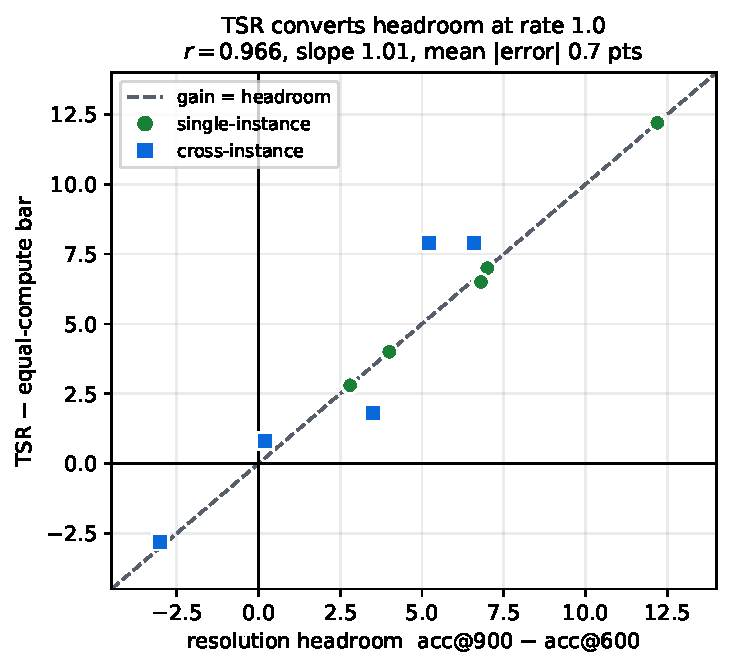
\includegraphics[width=0.52\textwidth]{figs/fig_identity.pdf}
\caption{\textbf{AVR is a resolution converter.} Its gain over the equal-compute bar tracks the headroom the
checkpoint already has, at rate $1.0$. The one cell where AVR loses is the one cell where the baseline itself is
worse at $900$ tokens than at $600$.}
\label{fig:identity}
\end{figure}


\begin{table}[h]\centering\small
\caption{AVR's gain against the headroom $\mathrm{acc}(900)-\mathrm{acc}(600)$, for the ten stratum-cells that
carry the \texttt{uniform@900} diagnostic. Pearson $r=0.966$, OLS slope $1.01$, mean
$|{\rm gain}-{\rm headroom}|=0.7$ points. Headroom is measurable from two baseline runs with no method involved.}
\begin{tabular}{llcc}
\toprule
cell & stratum & AVR $-$ bar & headroom\\
\midrule
\multirow{2}{*}{\vstar\ Qwen2.5-VL-7B} & single & \gd{$+12.2$}~\ok & $+12.2$\\
 & cross & $+7.9$ & $+5.2$\\
\multirow{2}{*}{\vstar\ Qwen3-VL-8B} & single & $+7.0$ & $+7.0$\\
 & cross & \gd{$+7.9$}~\ok & $+6.6$\\
\multirow{2}{*}{HR-4K Qwen3-VL-2B} & single & \gd{$+4.0$}~\ok & $+4.0$\\
 & cross & $-2.8$ & $-3.0$\\
\multirow{2}{*}{HR-4K Qwen2-VL-7B} & single & $+2.8$ & $+2.8$\\
 & cross & $+0.8$ & $+0.2$\\
\multirow{2}{*}{HR-8K Qwen3-VL-2B} & single & \gd{$+6.5$}~\ok & $+6.8$\\
 & cross & $+1.8$ & $+3.5$\\
\bottomrule
\end{tabular}\label{tab:identity}
\end{table}

The identity also holds where it predicts \emph{nothing}. Applying AVR to a crop rather than to the full image
gives eight further cells whose headroom is near zero; gain tracks headroom there with $r=0.911$ and slope $1.03$
(mean error $0.40$ points), and AVR correctly does nothing. Across both settings the identity is supported on
$18$ stratum-cells, and it is the only component of this work that predicted a negative result before we ran it.

Two consequences. First, the sign of the gain is predictable before deployment: the one cell where AVR loses
(HR-4K cross-instance) is the one cell where the baseline itself is worse at $900$ tokens than at $600$, so nothing
was available to convert. Second, the pruning contributes nothing on its own. Comparing AVR against \texttt{uniform@900}, which encodes at the
same resolution and prunes nothing, the two agree within $0.5$ points in $7$ of the $10$ cells
($+0.0$, $+0.0$, $+0.0$, $+0.0$, $+0.2$, $+0.5$, $-0.2$). In two more the pruned arm is \emph{ahead}, by $+1.3$ and
$+2.6$, which we read as noise rather than a benefit of pruning. Exactly one cell shows a real cost: HR-8K
cross-instance at $-1.8$ [$-3.2,-0.5$], the only measurable price of discarding $90\%$ of visual tokens anywhere in
this work. Pruning at the boundary is therefore free everywhere we have measured it but that one cell. We
verified the pruning is applied rather than silently skipped at the distribution level: output probabilities change
on $99\%$ of items while the arg-max changes on $2\%$. The discarded tokens are inert, not absent.

\section{Claim-to-evidence map}\label{app:claims}

Every headline claim, its strongest evidence, and its model count. \emph{Intervention} means the claim was tested by
changing the model's computation (mask, patch, prune, ablate, oracle), not by observation alone. A claim is exported
only if it holds on two checkpoints.

\begin{table}[h]\centering\scriptsize
\setlength{\tabcolsep}{3pt}
\caption{Claims, evidence class, and the models on which the evidence was measured.}
\begin{tabular}{p{2.9cm}p{5.6cm}p{1.8cm}p{2.5cm}}
\toprule
claim & strongest evidence & class & models \\
\midrule
transport complete by $0.57\times$ depth & layer-wise and prefix/suffix attention masks; $36$-layer boundary from pruning cost & intervention & $2\times28$-layer masking; $36$-layer pruning \\
image-token values inert past the boundary & representation patching at L$\ge$16, at $300$ and $900$ tokens & intervention & $2$ models, both strata \\
answer position does not read the image & answer-row-only mask, all layers & intervention & $2$ models \\
depth choice dominates & crop at every layer's arg-max, end task & intervention & $2$ models \\
usable read-out band lies after transport & coverage curve, end-task sweep, location probe & measurement $+$ intervention & $2$ models (curve, probe) \\
ranking matters before the boundary only & probe vs random keep at L4; random $=$ attention at L16/L24; value patching & intervention & $2$ models \\
block mean fails on the item-independent component & nuisance ablation: $0.083{\to}0.438$, $0.292{\to}0.490$ & intervention & $2$ models \\
supervised depth weighting, not signed subtraction & non-negative fit retains the advantage ($44/43$ of $56$ coefficients zeroed); end task n.s. & intervention & $2$ models \\
DWA beats every published rule at equal compute & $9/9$ pooled paired contrasts & evaluation & $2$ models $\times$ $2$ benchmarks \\
AVR pruning is free & pruned vs unpruned @$900$; value patching at L16 & intervention & $2$ models \\
AVR's gain is resolution headroom & $10$-cell identity, $r=0.966$; distributional equivalence & accounting $+$ intervention & $4$ checkpoints \\
cropping helps single-instance, not cross & $14$-cell scope table $+$ oracle ceiling & evaluation $+$ intervention & $4$ checkpoints \\
a map-only gate removes the cross loss & $8$-cell policy table: AND of three label-free statistics; HR-4K cross $+0.8$/$+1.0$, \vstar\ both strata clear & evaluation & $2$ models $\times$ $4$ benchmarks \\
DWA matches native resolution at $14$--$18\%$ compute & end-task vs native & evaluation & $2$ models \\
placement is worth $>5\times$ the compute & oracle-crop arm beats native & intervention & $2$ models \\
\bottomrule
\end{tabular}\label{tab:claims}
\end{table}

\section{Scope and compute, as figures}\label{app:figs}

\begin{figure}[h]\centering
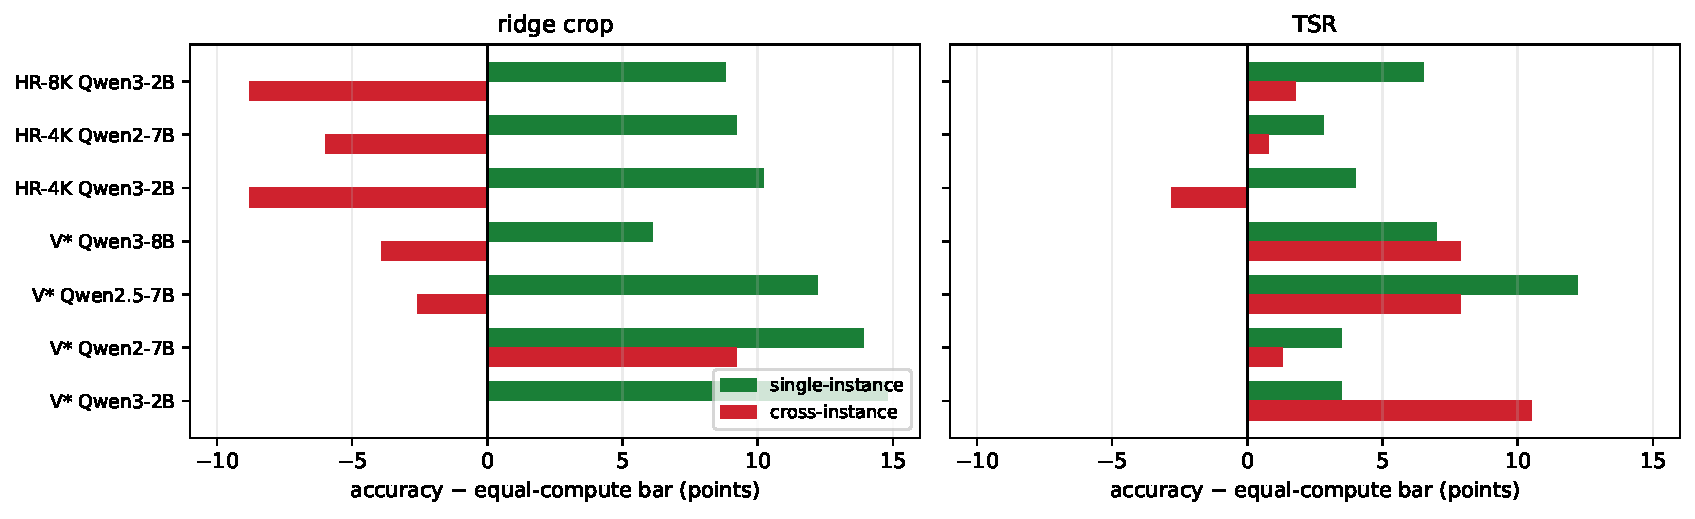
\includegraphics[width=\textwidth]{figs/fig_scope.pdf}
\caption{\textbf{The scope law.} Cropping is worth $+6$ to $+15$ points on single-instance questions in all seven
cells and is negative on cross-instance in six of them. AVR is positive on both strata in six of seven, and gives
up most of the single-instance gain to get there. The two policies are not variants of one method.}
\label{fig:scope}
\end{figure}

\begin{figure}[h]\centering
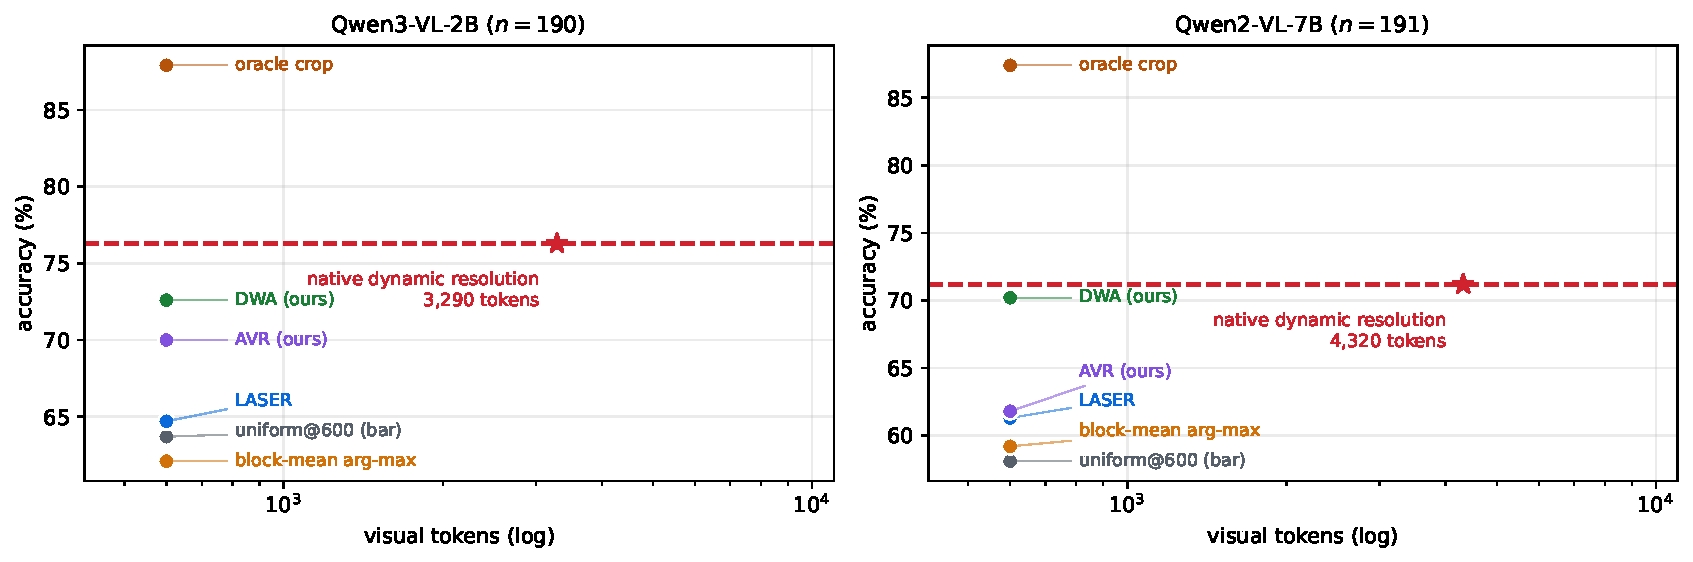
\includegraphics[width=\textwidth]{figs/fig_native.pdf}
\caption{\textbf{Accuracy against visual-token compute}, \vstar. The dashed line is the model run at its own
native dynamic resolution. Our two policies sit on it at $14$--$18\%$ of its compute; the published rules sit
significantly below it; and a perfectly placed $600$-token crop sits well above it. Placement is worth more than
$5$--$7\times$ the tokens.}
\label{fig:native}
\end{figure}

\section{Mechanism: three stages, three interventions}\label{app:mech}

\begin{figure}[h]\centering
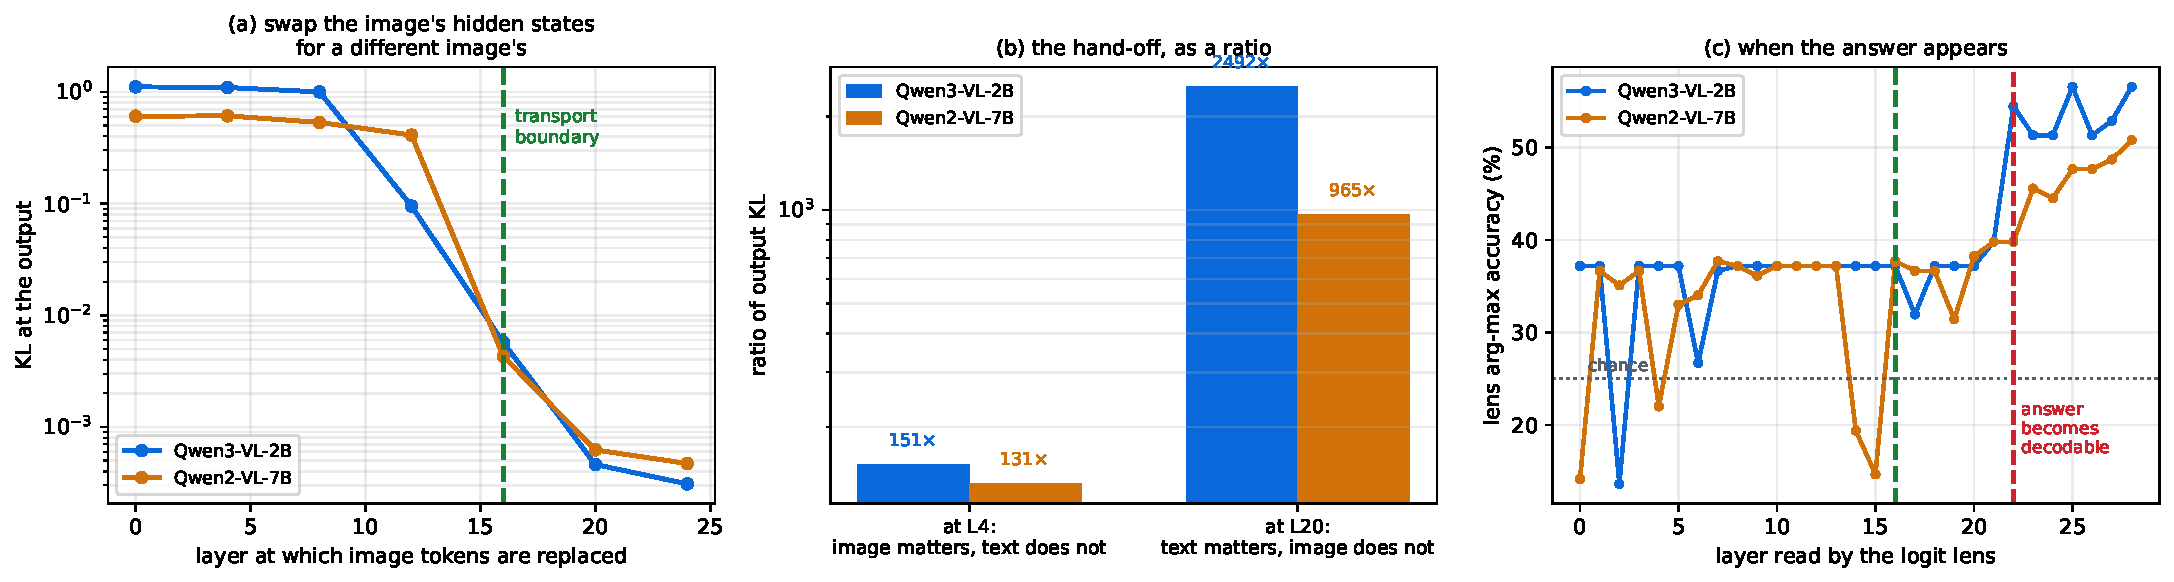
\includegraphics[width=\textwidth]{figs/fig_mechanism.pdf}
\caption{\textbf{(a)} Replacing the image tokens' hidden states at layer $\ell$ with a different image's: the
output effect falls three orders of magnitude across the boundary. \textbf{(b)} The hand-off as a ratio: early,
the image dominates and the text is inert; late, exactly the reverse. \textbf{(c)} Logit lens at the answer
position: the correct option becomes decodable only in the last quarter of the stack.}
\label{fig:mech}
\end{figure}

Each row of Table~\ref{tab:stages} is measured by a different intervention, so no stage rests on the method that
found another.

\begin{table}[h]\centering\small
\caption{The three stages. Every number is measured on both core checkpoints.}
\setlength{\tabcolsep}{4pt}\begin{tabular}{p{2.2cm}p{1.35cm}p{2.8cm}p{5.5cm}}
\toprule
stage & layers & measured by & evidence\\
\midrule
image $\to$ text transport & L0--L16 & attention masking; hidden-state patching & suffix masks cost nothing from L16 ($0.014$, $0.029$); the patch effect falls $17\times$ and $96\times$ between L12 and L16\\
question-conditioned read-out & L17--L21 & end-task accuracy by read-out depth & crop accuracy spans $34.6$--$70.2$, peaking at L17; no layer inside the window beats not cropping\\
answer formation & L22+ & logit lens & lens accuracy steps $+18.0$ [$+8.7,+27.0$] and $+14.2$ [$+7.2,+21.3$] above its early plateau\\
\bottomrule
\end{tabular}\label{tab:stages}
\end{table}

The logit lens is computed with the final norm applied to intermediate layers only; applying it to the last hidden
state as well double-normalises and corrupts that layer alone, which cost us a retracted result earlier in this
project. We assert per run that our last-layer read-out matches the true logits.

A fourth, independent technique places the read-out band in the same spot: a ridge probe from the
answer-position state to the target's location rises across the transport window and peaks at L18--19 (Qwen3,
$r=+0.635$) and L18 (Qwen2, $+0.603$).

\paragraph{The channel and the values.} Masking blocks the text$\to$image attention \emph{channel}; it does not
show that the image information is absent from the residual stream. Replacing the image tokens' hidden states
with a donor image's (same question, same token budget) closes that gap. The effect falls three orders of
magnitude across the boundary, and both pre-registered controls behave as required: patching the image at L4 is
large, patching text at L20 is large.

\begin{table}[t]
\caption{Representation patching: replace the image tokens' hidden states at one layer's output with a donor
image's; KL at the output and answer flips. Text controls patch text-token states at the same depth.}
\label{tab:patch}
\begin{center}
\small
\begin{tabular}{lcc}
\multicolumn{1}{c}{\bf patch site} &\multicolumn{1}{c}{\bf Qwen3-VL-2B KL (flips)} &\multicolumn{1}{c}{\bf Qwen2-VL-7B KL (flips)}
\\ \hline \\
image L0 & 1.758 (61.7\%) & 0.800 (60.0\%)\\
image L4 (control C1) & 1.766 (63.3\%) & 0.798 (58.3\%)\\
image L8 & 1.622 (60.0\%) & 0.657 (60.0\%)\\
image L12 & 0.134 (16.7\%) & 0.517 (51.7\%)\\
image L16 & 0.009 (3.3\%) & 0.005 (5.0\%)\\
image L20 & 0.0005 (0\%) & 0.0008 (1.7\%)\\
image L24 & 0.0003 (0\%) & 0.0006 (1.7\%)\\
text L4 & 0.009 (5.0\%) & 0.006 (3.3\%)\\
text L20 (control C2) & 1.834 (63.3\%) & 0.802 (60.0\%)\\
\end{tabular}
\end{center}
\end{table}

The late-image arm lands exactly on the text-L4 noise floor ($0.009$ vs $0.009$ on Qwen3; $0.005$ vs $0.006$ on
Qwen2), and the two controls invert cleanly across depth: at L4 the image matters $151\times$/$131\times$ more
than the text, at L20 the text matters $2492\times$/$965\times$ more than the image. Two different
interventions, two checkpoints, one boundary.

\paragraph{The boundary at the AVR operating point.} AVR encodes at $900$ tokens and prunes at the boundary, so
inertness must hold on the unpruned $900$-token pass. Injecting donor values at the layer's output:

\begin{table}[t]
\caption{Value inertness at $900$ tokens (Qwen3-VL-2B, $n=191$): donor hidden states at the layer's output.}
\label{tab:inert900}
\begin{center}
\small
\begin{tabular}{lcc}
\multicolumn{1}{c}{\bf patch at 900 tokens} &\multicolumn{1}{c}{\bf mean KL} &\multicolumn{1}{c}{\bf answer flips}
\\ \hline \\
dropped positions @L16 (810 of 900) & 0.0022 & 1.0\%\\
kept positions @L16 (90 of 900) & 0.0065 & 3.1\%\\
dropped positions @L8 (transport window) & 0.3407 & 20.9\%\\
\end{tabular}
\end{center}
\end{table}

At the boundary the values are inert whether or not they are the ones AVR keeps; inside the transport window
the same intervention moves one answer in five.

\paragraph{The cost of misplacing the boundary.} Pruning is free at the boundary and expensive before it. With
the same number of tokens dropped and a large negative attention bias on the dropped columns from layer $K$
onward (functionally FastV's rule):

\begin{table}[t]
\caption{Pruning depth and selection. V*Bench, $n=191$; every arm prunes the same count.}
\label{tab:prunedepth}
\begin{center}
\small
\begin{tabular}{lccc}
\multicolumn{1}{c}{\bf keep} &\multicolumn{1}{c}{\bf random} &\multicolumn{1}{c}{\bf layer-2 (FastV default)} &\multicolumn{1}{c}{\bf late read-out (L16--26)}
\\ \hline \\
10\% & 38.2\% & 34.6\% & 56.0\%\\
25\% & 41.4\% & 40.3\% & 58.1\%\\
50\% & 47.1\% & 52.9\% & 55.5\%\\
\end{tabular}
\end{center}
\end{table}

No pruning is $56.5\%$. Ranking at layer 2 costs $22.0$ points against no pruning and is $3.7$ points
\emph{worse than random}; the late read-out deletes $90\%$ of visual tokens at $-0.5$ points [$-5.8,+4.7$] and
the learned criterion at $+2.1$ [$-2.6,+6.8$]. The collapse replicates on Qwen2-VL-7B (late over layer-2
$+11.5$ [$+4.2,+18.8$] at $10\%$ keep; layer-2 is $4.7$ points below random) and is larger on general VQA:
layer-2 against random is $-15.0$ [$-22.0,-7.5$] on POPE and $-25.5$ [$-33.0,-18.0$] on MMBench.

\paragraph{Selection stops mattering at the boundary.} Before the boundary, which tokens survive matters: a
layer-4 probe beats random keep by $+8.4$ [$+2.1,+15.2$] and $+8.9$ [$+2.6,+15.2$] at $25\%$ keep. At and after
it, the choice is irrelevant: random keep matches attention keep on both models at every keep ratio tested,
and pruning is free ($0.0$--$0.5$ points in $9$ of $10$ cells). The boundary is not merely where pruning
becomes cheap; it is where selection ceases to matter.

\section{Propositions, and what validates them}\label{app:theory}

We state four theorems, three propositions and two lemmas. They are not deep results --- two are tail-dominance and
sufficiency statements, two are information bounds, and the lemmas are one-line linear algebra --- but each makes a
prediction that could have failed on data, and we report where they hold approximately rather than exactly. All measurements are out-of-fold on both core
checkpoints; $n=126$ (modal grid) for coverage, $n=191$ for end-task and distributional tests.

\textbf{Setup.} For item $i$, layer $\ell$, cell $c$, let $A_\ell^{(i)}(c)\ge0$ be the last-prompt-token attention
mass on cell $c$, row-normalised so $\sum_cA_\ell^{(i)}(c)=1$. Write $m_\ell=\mathbb{E}_iA_\ell^{(i)}$ for the
\emph{item-mean} (item-independent) map and $A_\ell^{(i)}=m_\ell+U_\ell^{(i)}$, so $\mathbb{E}_iU_\ell^{(i)}=0$.

\begin{theorem}[Tail dominance of the conventional read-out]\label{thm:tail}
Write each depth's per-cell score as $x_\ell(c)=m_\ell(c)+u_\ell(c)$ with $u_\ell$ zero-mean over items, and put
$\Delta_B=\max_c\sum_{\ell\in B}m_\ell(c)-\mathrm{med}_c\sum_{\ell\in B}m_\ell(c)$. The block read-out returns
$\arg\max_c\sum_{\ell\in B}x_\ell(c)$.
\begin{enumerate}\itemsep0pt
\item[(i)] If $\Delta_B$ exceeds the range of $\sum_{\ell\in B}u_\ell$, the arg-max is
  $\arg\max_c\sum_B m_\ell$ for \emph{every} item: a fixed cell independent of the image.
\item[(ii)] Equal-weight positive averaging cannot escape (i) at \emph{any} band width: the $m_\ell$ leads are
  sign-aligned across depth, so $\Delta_B$ is superadditive in $B$.
\item[(iii)] Any per-cell rescaling that equalises $m$ across cells --- in particular dividing by an estimate of
  $m$ --- removes the dominance without using labels.
\end{enumerate}
\end{theorem}
\begin{proof}
(i) If the deterministic part's lead exceeds the total variation the item-specific part can supply, it decides the
maximum. (ii) Each summand contributes its $m_\ell$ lead with the same sign, so $\Delta_B$ is superadditive; whether
$\Delta_B/\sigma_B$ rises or falls depends on the covariance of the $u_\ell$, and the claim is only that it does not
reach the $O(1)$ regime in which $\sum_B u_\ell$ could decide the arg-max. (iii) Immediate from (i) applied to the
rescaled scores.
\end{proof}

\begin{lemma}[Leakage decomposition]\label{lem:leak}
For every weight vector $w$, $\sum_\ell w_\ell A_\ell^{(i)}=L(w)+\sum_\ell w_\ell U_\ell^{(i)}$ with
$L(w)=\sum_\ell w_\ell m_\ell$ independent of $i$. The item-independent component of the score is exactly $L(w)$.
\end{lemma}
\begin{proof}
Substitute the decomposition and rearrange. $L(w)$ carries no $i$-dependence, so its ranking of cells is identical
for every item.
\end{proof}

\begin{lemma}[Non-negative filters cannot cancel a common prior]\label{lem:nn}
If the item-mean maps are rank-one across depth, $m_\ell=\alpha_\ell\mu$ with $\mu\neq0$ and $\alpha_\ell>0$, then
$L(w)=(\alpha^\top w)\mu$. Hence $L(w)=0$ iff $\alpha^\top w=0$; no non-zero $w\ge0$ achieves zero leakage.
\end{lemma}
\begin{proof}
Linearity, then $\alpha^\top w=\sum_\ell\alpha_\ell w_\ell>0$ whenever $w\ge0$, $w\neq0$.
\end{proof}

\emph{Every part is measured, and the measurements decide between accounts that (ii) alone cannot separate.}
On the items the block mean gets wrong, the cell it selects sits at the \textbf{100th percentile} of the
item-independent map --- on both checkpoints, on every failure. It is not mis-weighting evidence; it is returning
the raster sink. Consistent with (ii), $\Delta_B/\sigma_B$ measured over band widths $1$ to $11$ stays between $10.2$ and $16.6$
on one checkpoint and between $7.0$ and $15.1$ on the other --- always an order of magnitude above the regime
where the item-specific term could win, so no amount of averaging rescues the rule. The ratio \emph{rises} with
width on the first checkpoint and \emph{falls} on the second, so we claim only that averaging never escapes, not
that wider is monotonically worse. What is common to both is that the deployed eleven-wide band is worse than the
best narrower band ($0.418\to0.083$ and $0.390\to0.297$), and that its last-column rate is higher there
($17.5\to91.3\%$ and $45.2\to62.7\%$). Consistent with (iii), an \emph{unsupervised} correction --- divide each cell by its value on a typical
item, then take the arg-max --- lifts coverage from $0.083$ to $0.408$ and from $0.292$ to $0.504$, reaching
$71\%$ and $86\%$ of what the fitted read-out achieves, and drops the last-column rate to $2.4\%$ and $0.0\%$
against a $4.8\%$ chance rate, with no ring mask.

\emph{And it buys nothing at the end task, which bounds what this proposition explains.} Run as a placement rule
and answered, the same label-free correction scores $59.7\%$ and $61.3\%$ against the block mean's $62.3\%$ and
$59.2\%$: $-2.6$ [$-7.9,+2.6$] and $+2.1$ [$-3.1,+7.3$], neither clear of zero, and it does not beat not cropping
at all. DWA beats it by $+13.1$ [$+5.8,+20.4$] and $+8.9$ [$+2.6,+15.2$], clear on both checkpoints. So the
proposition explains why the conventional read-out \emph{places} badly, and a label-free fix repairs the
placement, but repairing placement is not what the fitted read-out is selling. Its end-task advantage survives
after the placement failure has been removed by other means, and we do not yet have a mechanism for that
remainder. This is also the largest coverage-to-accuracy gap we have measured --- $66$--$70\%$ of the coverage gap
closed, none of the accuracy gap --- and it is a caution that applies to our own use of coverage in this section,
not only to prior work.

\emph{What the fit adds, and why its sign does not matter.} Because the features are log-attention, a weight
vector summing to zero computes a \emph{ratio} across depths, which cancels any per-cell factor common to all
layers; the fitted weights are close to that, with $|\sum_\ell w_\ell|/\sum_\ell|w_\ell| = 0.126$ and $0.225$.
But that is not the only route. Sink dominance itself varies $3.2\times$ and $4.4\times$ across depth, and the
least-dominated depths are exactly the read-out band, so a strictly non-negative read-out can escape by
\emph{selecting} those depths rather than by cancelling anything. Both routes are available, which is why
constraining every weight to be non-negative costs nothing while zeroing $44$ and $43$ of $56$ coefficients. The
item-mean maps are approximately rank-one (leading eigenvalue share $0.86$ and $0.77$), and in map space the
non-negative constraint costs only $0.044$ and $0.002$ mean coverage: the sign of the fitted weights is an artefact
of ridge collinearity between adjacent layers, not the mechanism. We do
not claim the fitted weights track dominance depth-by-depth: that correlation is only $+0.171$ and $+0.131$. The
supported statement is that the failure is tail dominance, that it has an unsupervised fix which recovers most of
the gap, and that supervision buys the remaining $14$--$29\%$.

\emph{A refinement the theory predicted, which failed.} If what remains after dividing out $m$ were
heteroscedastic across cells, the right label-free statistic would be the studentised one, $(x(c)-m(c))/s(c)$. We
pre-registered that it would beat the plain ratio. It does not, on either checkpoint ($-0.015$ and $-0.028$), and
it closes $63\%$ and $61\%$ of the gap against the plain ratio's $66\%$ and $70\%$. The proposition therefore
explains the failure and supplies a label-free correction, but does not yet predict a better one: the residual
that supervision buys is not simple heteroscedasticity.

\emph{Two accounts we tested first and rejected.} That signed weights cancel a common nuisance: refuted, since
non-negative fits lose nothing and the orthogonality the argument needs measures $+0.431$ and $+0.388$ rather than
zero. That the fit is a matched filter over depth, weighting by per-layer signal-to-noise: refuted, one of two on
each of its predictions, and wrong in kind --- the block mean already retains $77\%$ of attainable signal-to-noise
on both models while its coverage is several times worse, and a mean-based quantity cannot explain an arg-max
failure.

\begin{theorem}[A single-depth read-out is lossy unless that depth is sufficient]\label{thm:suff}
Let $c^\star$ be the cell containing the evidence and $A=(A_1,\dots,A_L)$ the depth profile. For any rule
$\hat c=g(A_\ell)$ reading a single layer: (i) $c^\star\to A\to A_\ell\to\hat c$ is a Markov chain, so
$I(c^\star;\hat c)\le I(c^\star;A_\ell)\le I(c^\star;A)$; (ii) the right inequality is an equality iff
$c^\star\perp A\mid A_\ell$, i.e.\ $A_\ell$ is sufficient for $c^\star$ within the profile; (iii) by Fano,
$\Pr[\hat c\neq c^\star]\ge(H(c^\star)-I(c^\star;A_\ell)-1)/\log|\mathcal{C}|$.
\end{theorem}

\begin{proof}
$A_\ell$ is a coordinate projection of $A$ and $\hat c$ is post-processing of $A_\ell$, so the chain holds and
the data-processing inequality applies along each link, giving (i). For (ii),
$I(c^\star;A)-I(c^\star;A_\ell)=I(c^\star;A\mid A_\ell)\ge0$ by the chain rule, with equality exactly under
conditional independence. (iii) is Fano applied to that chain.
\end{proof}

Theorem~\ref{thm:suff} is vacuous until sufficiency is decided, and sufficiency is an empirical property of a
given model, so we test its equality condition. If $A_\ell$ were sufficient its arg-max would be correct
wherever any layer's is, so the best single depth would match the family's envelope. Cropping at every one of
the $28$ layers' arg-max and answering gives:

\begin{table}[h]\centering\small
\setlength{\tabcolsep}{5pt}
\caption{The sufficiency test at the end task. A sufficient layer would make the first two columns equal.}
\begin{tabular}{lccccc}
\toprule
& best depth & some depth & gap & every depth & spread over depth\\
\midrule
Qwen3-VL-2B & $70.2$ & $\mathbf{95.3}$ & $+25.1$ & $5.2$ & $34.6$--$70.2$\\
Qwen2-VL-7B & $62.8$ & $\mathbf{89.5}$ & $+26.7$ & $9.9$ & $36.1$--$62.8$\\
\bottomrule
\end{tabular}\label{tab:suff}
\end{table}

Sufficiency is rejected on both checkpoints by $25$ and $27$ points. The escape is to read every depth: DWA
is $+2.6$ [$-3.7,+8.9$] and $+7.3$ [$+1.0,+13.1$] against the best single depth --- a depth chosen \emph{on
the test set}, so an optimistic baseline --- clear on one checkpoint and matching on the other, while the
published fixed choice sits $31.9$ and $19.9$ points below that oracle. The scope of the test is stated: the
envelope is measured over the arg-max read-out family, which is the class a depth-selection rule chooses among,
not over all measurable functions of $A$.

\begin{theorem}[Decoding bound, and a certified gap for the conventional read-out]\label{thm:info}
For any read-out decision $\hat c$ of a per-cell score and target cell $T$:
(i) $I(\hat c;T)\le H(\hat c)\le\log|\mathcal C|$;
(ii) $I(\hat c;T)\ge H(T)-H_b(P_e)-P_e\log(|\mathcal C|-1)$ with $P_e=\Pr[\hat c\ne T]$;
(iii) if $\hat c$ is constant then $I(\hat c;T)=0$.
\end{theorem}
\begin{proof}
(i) $I(\hat c;T)=H(\hat c)-H(\hat c\mid T)\le H(\hat c)\le\log|\mathcal C|$. (ii) Fano's inequality.
(iii) $H(\hat c)=0$, so (i) gives $I=0$.
\end{proof}

The bounds are exact and directly measurable, and the same maps admit an oracle decision that \emph{is} the target,
so $I(\text{oracle};T)=H(T)=6.06$ bits on the modal-grid items. The conventional read-out does not reach that: the
literal block mean (no ring mask) has decision entropy $1.02$ and $3.46$ bits on the two checkpoints and lands in
the grid's last column on $84.8\%$ and $61.8\%$ of the full item set, so it can carry at most that much --- a
certified gap of $\ge5.0$ and $\ge2.6$ bits. The ring mask restores the baseline's decision entropy ($6.30$/$4.60$
bits) but not its accuracy; the fitted read-out attains the same entropy with higher coverage ($0.605$/$0.581$
against $0.459$/$0.402$). The failure is in the decoder, not the representation. Two consequences. The information
a decision can carry is raised only by making it \emph{varied} or \emph{accurate} --- the bounds never mention
cancellation --- so a non-negative depth fit reaches the same terms by selecting the depths where the
item-independent component is least dominant (\S\ref{sec:dwa_method}). And the depth \emph{ordering} changes both terms
while the sign of the weights does not.

\begin{theorem}[The information horizon]\label{thm:horizon}
Suppose the visual-token values after layer $p$ are output-invariant:
$I(V_{>p};Y\mid\text{state}_p)=0$ (value-inertness). Then (i) pruning to any keep-set loses no answer
information; (ii) AVR's gain over the bar $E_0$ is the resolution information gain
$\mathrm{acc}(E)-\mathrm{acc}(E_0)$, bounded by $I(X;Y)-I(Z_{E_0};Y)$; and (iii) the information-bearing depth is
$p+1$ layers, so the affordable resolution multiplier is $N/(p+1)=1.647\times$ over uniform-depth encoding.
\end{theorem}
\begin{proof}
(i) The premise makes the answer conditionally independent of those values given the state at $p$, and the keep-set
is a function of them. (ii) Pruning is information-free by (i), so AVR and uniform encoding at $E$ induce the same
distribution; the data-processing inequality bounds the remaining difference by the information the bar's encoding
fails to carry. (iii) Token-layer accounting with the information-bearing depth.
\end{proof}

The premise is measured with its violation bounded by Pinsker, $\mathrm{TV}\le\sqrt{\mathrm{KL}/2}$: at the
boundary the answer distribution depends on the token values by at most $0.033$--$0.044$ in total variation, while
the same patch one window earlier moves it by $0.36$--$0.41$ (Appendix~\ref{app:mech}). The horizon is sharp, and it
is the same $0.57\times$ depth the masking experiments locate. The conclusion is what
Appendix~\ref{app:identity} tests: gain tracks headroom with $r=0.966$ over ten cells, and again with $r=0.911$
over eight further cells whose headroom is near zero, where it correctly predicts that AVR does nothing.
\emph{Where it is only approximate:} the premise holds to KL~$\approx5\times10^{-4}$, not to zero, so the
conclusion is approximate too. Measured slippage is at most $0.5$ points in seven of ten cells and $-1.8$ in one.
The theorem's real content is that the \emph{choice} of keep-set is irrelevant, which is why random keep matches
attention keep on $96.3\%$ of items.

\begin{proposition}[The budget determines the affordable resolution]\label{prop:budget}
\emph{Pruning to a fraction $k$ at layer $P$ of $N$ costs $\mathrm{TL}=E(P{+}1)+kE(N{-}1{-}P)$ token-layers.
Matching a uniform bar of $B$ tokens gives $E^\star = BN/\big((P{+}1)+k(N{-}1{-}P)\big)$.}
With $B=600$, $N=28$, $P=16$, $k=0.1$ this is $E^\star=928$, a $1.55\times$ resolution multiplier. We ran $E=900$,
$97\%$ of the optimum, and realised $96$--$100\%$ of the bar. This is arithmetic; we state it because it is the
design equation, and because it says the multiplier is fixed by the boundary's depth fraction rather than chosen.
\end{proposition}

\begin{proposition}[Value-inertness implies selection irrelevance]\label{prop:sel}
Suppose that for every subset $D$ of visual positions, replacing the hidden values of $D$ at layer $p$ with
arbitrary donor values leaves the option distribution unchanged. Then for any two keep-sets $D_1,D_2$ of equal
size, the models $U_E\circ P_{D_1}$ and $U_E\circ P_{D_2}$ induce the same distribution: every ranking rule is
equivalent.
\end{proposition}
\begin{proof}
The premise makes the output invariant to the values of any subset of visual positions at layer $p$. The kept set
is such a subset, so no choice of kept set can change the distribution.
\end{proof}
\emph{Validation.} On the unpruned $900$-token pass at the boundary (L16, Qwen3, $n=191$), replacing the hidden
states of the $810$ pruned positions with another image's gives KL $0.0022$ ($1.0\%$ flips) and replacing the $90$
kept positions gives KL $0.0065$ ($3.1\%$); the same patch at L8 gives $0.341$ ($20.9\%$). Qwen2 replicates
($0.0038$/$3.7\%$ and $0.0027$/$0.5\%$ at L16; $0.2622$/$29.8\%$ at L8), so the premise holds on both models.

\begin{proposition}[A single window cannot serve two distant sites]\label{prop:window}
\emph{A window of side $W$ contains at most one of two evidence sites separated by more than $W$.}
Trivial, and it is not the interesting part. The interesting part is empirical: with \emph{perfect} placement,
cross-instance error stays at $25\%$ and $22\%$ against $3.5\%$ and $6.1\%$ for single-instance, and two
full-resolution crops covering both objects still score $-2.6$ and $-3.9$ against one. The residual is not a
perceptual failure, so no reallocation of perceptual resource reaches it --- which is why the scope law is a
property of the question type and not of the method.
\end{proposition}

\section{Additional visualisations}\label{app:vis}


\begin{figure}[h]\centering
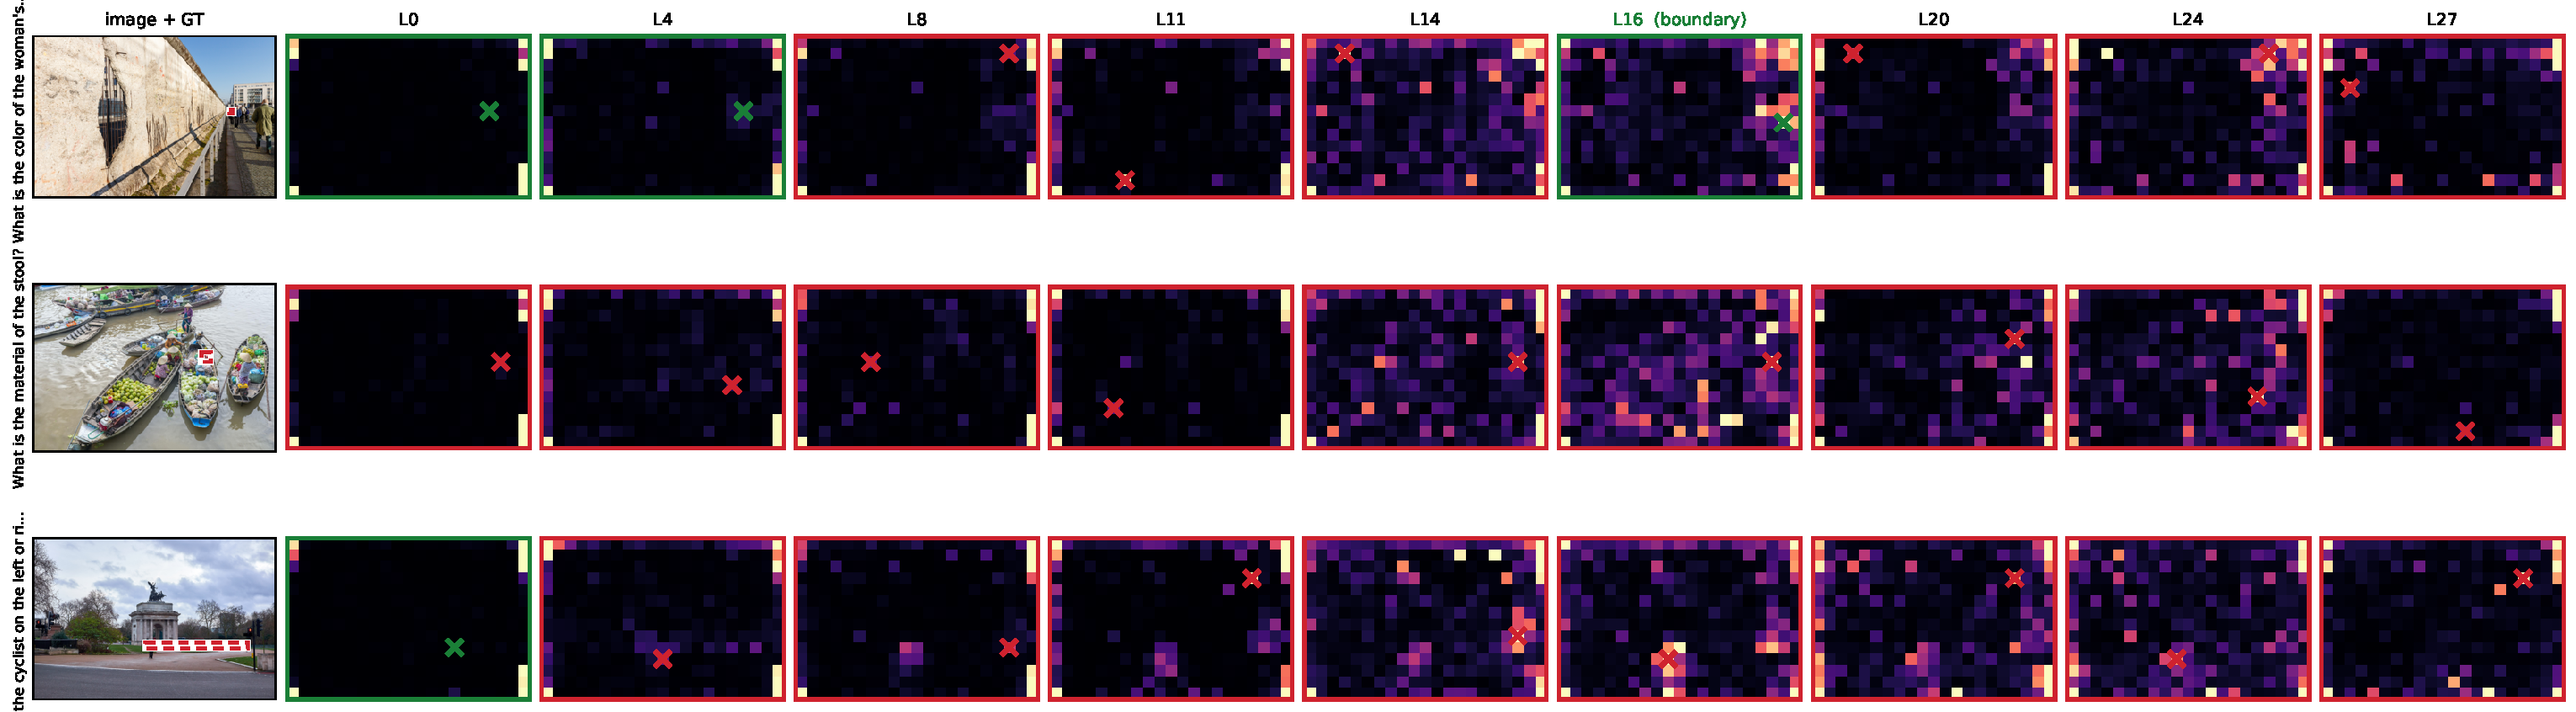
\includegraphics[width=\textwidth]{figs/fig_layer_disagreement.pdf}
\caption{\textbf{The same image, the same question, a different answer about where to look at every depth.}
Each panel is one layer's attention over image cells (colour clipped at the 98th percentile so the serialisation
sink does not wash out the structure); the cross is that layer's ring-masked arg-max, green where the resulting
crop would cover the evidence and red where it would not. Nothing about the input changes across a row. Only the
read-out depth does.}
\label{fig:layerdis}
\end{figure}

\begin{figure}[h]\centering
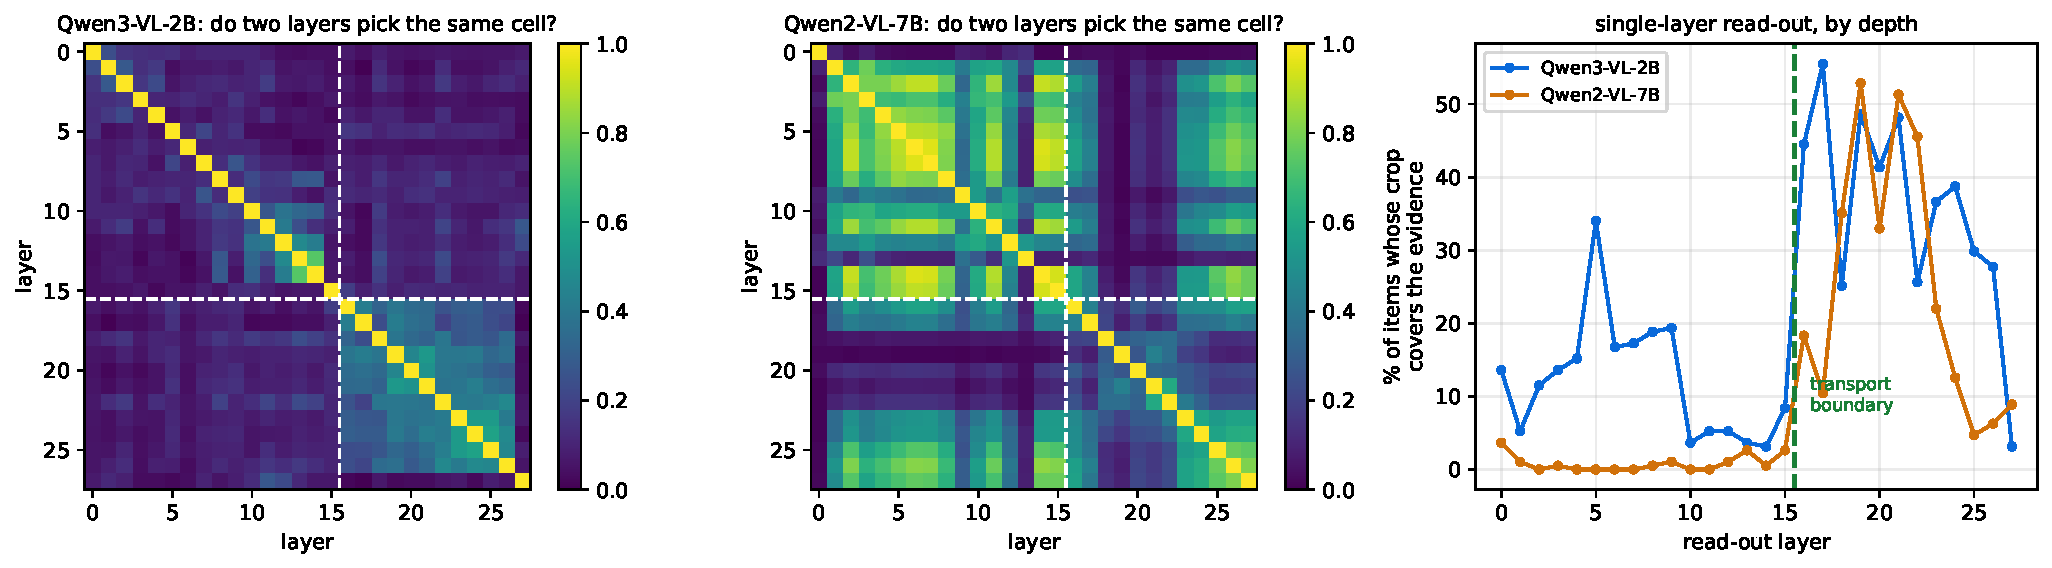
\includegraphics[width=\textwidth]{figs/fig_layer_agreement.pdf}
\caption{\textbf{Left, centre: two layers rarely choose the same cell.} Mean off-diagonal agreement is $13.8\%$
and $38.1\%$; the block structure splits at the transport boundary (dashed). \textbf{Right: and only the layers
after the boundary are worth reading.} The fraction of items whose single-layer crop covers the evidence is at or
below $20\%$ everywhere before the boundary, jumps immediately after it, and decays again toward the output. This
is the paper's central claim in one curve: the usable placement signal exists only after transport has finished.}
\label{fig:layeragree}
\end{figure}

\begin{figure}[h]\centering
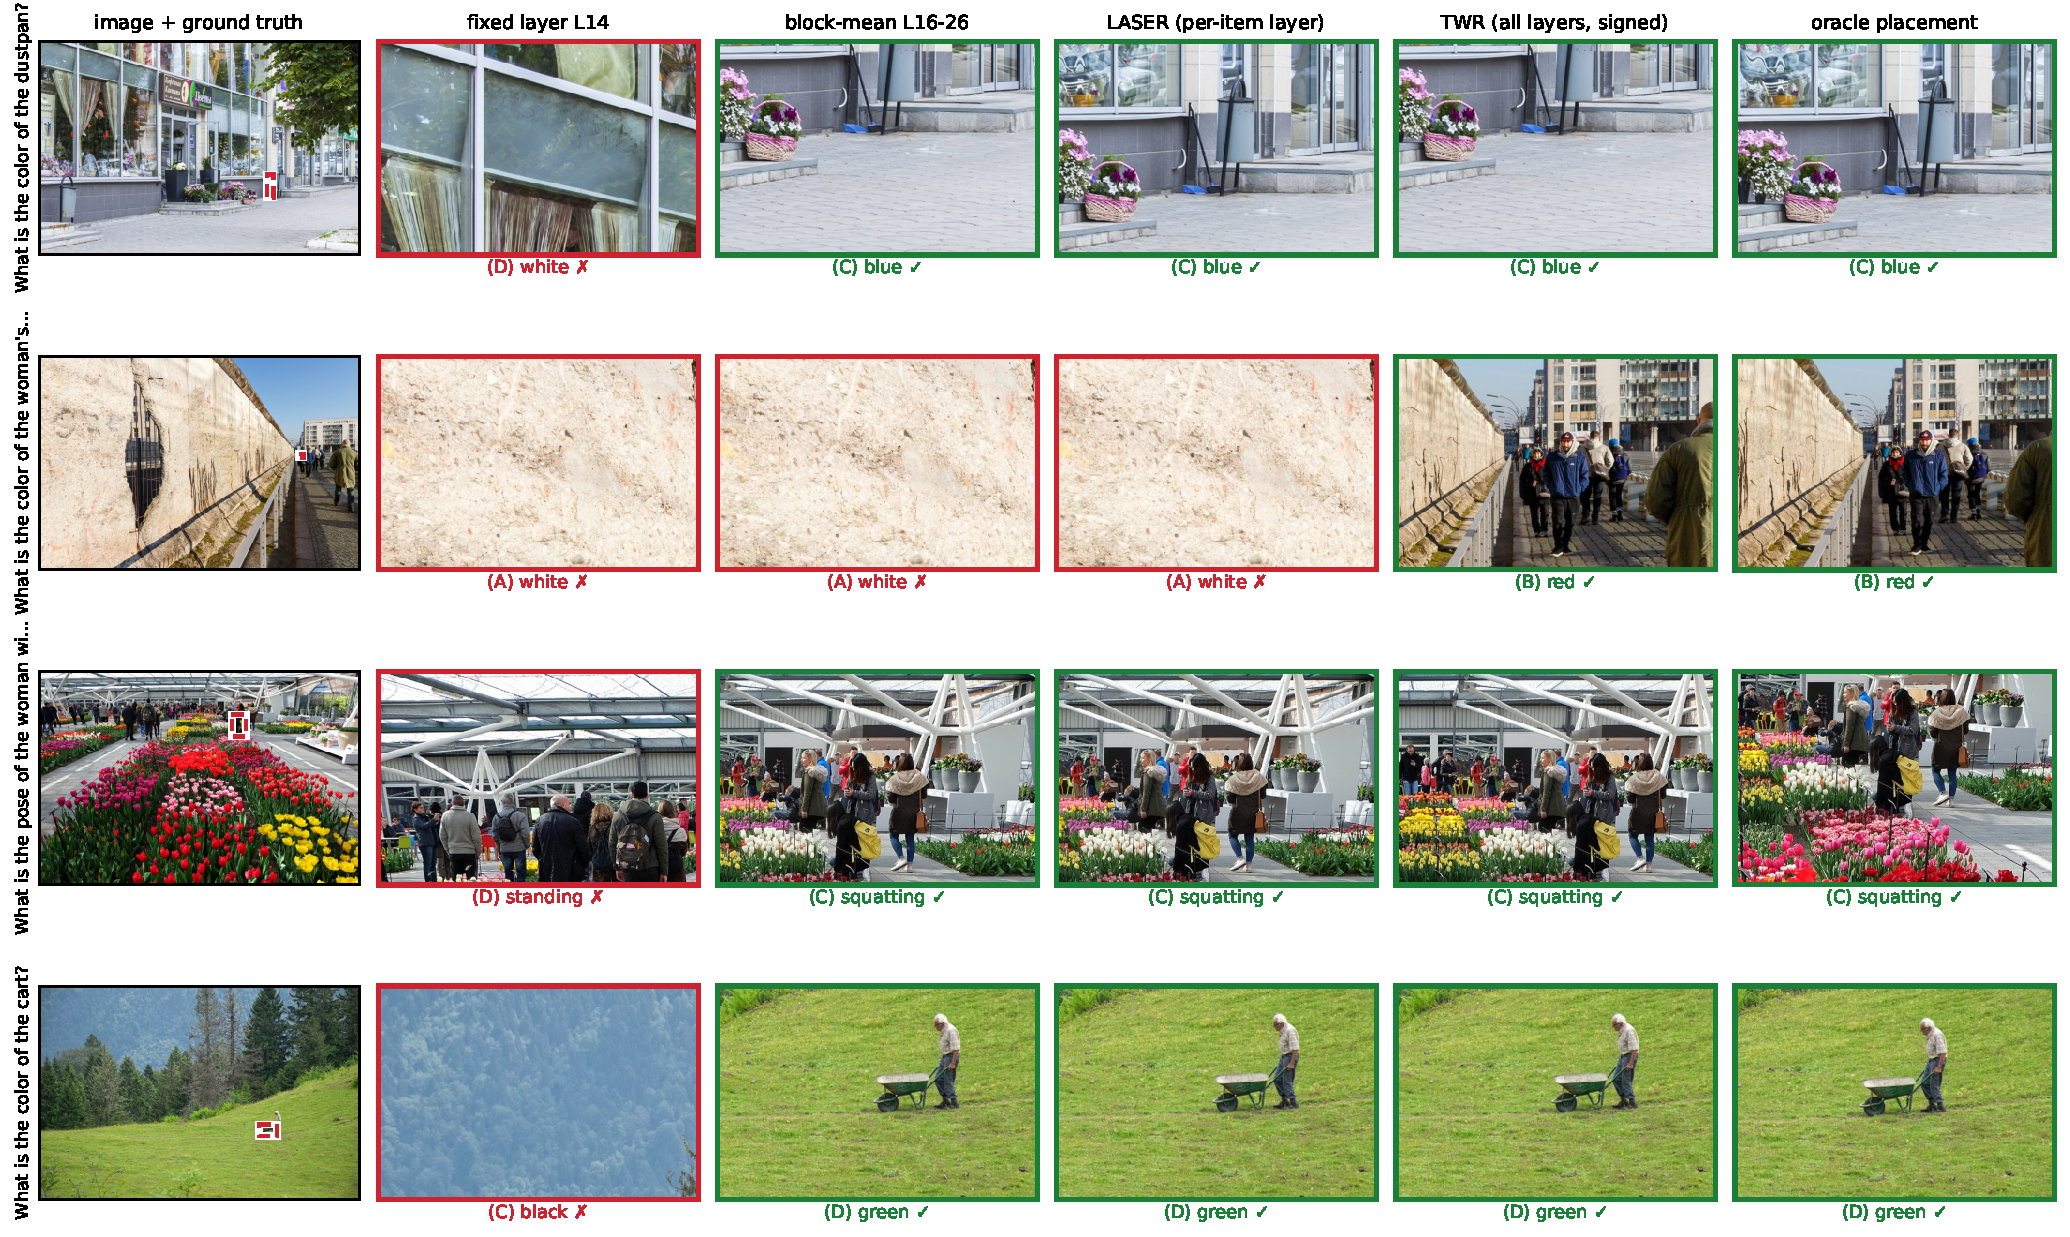
\includegraphics[width=\textwidth]{figs/fig_rule_comparison.pdf}
\caption{\textbf{Five placement rules, same items, same budget.} Selection rule: single-instance items on which
the oracle crop is correct, so the ceiling behaves like a ceiling, and on which DWA is correct while the
fixed-layer rule is not; $61$ items qualify and the first four by question id are shown. The fixed mid-layer
recipe crops glass, masonry and sky.}
\label{fig:rulecmp}
\end{figure}

\begin{figure}[h]\centering
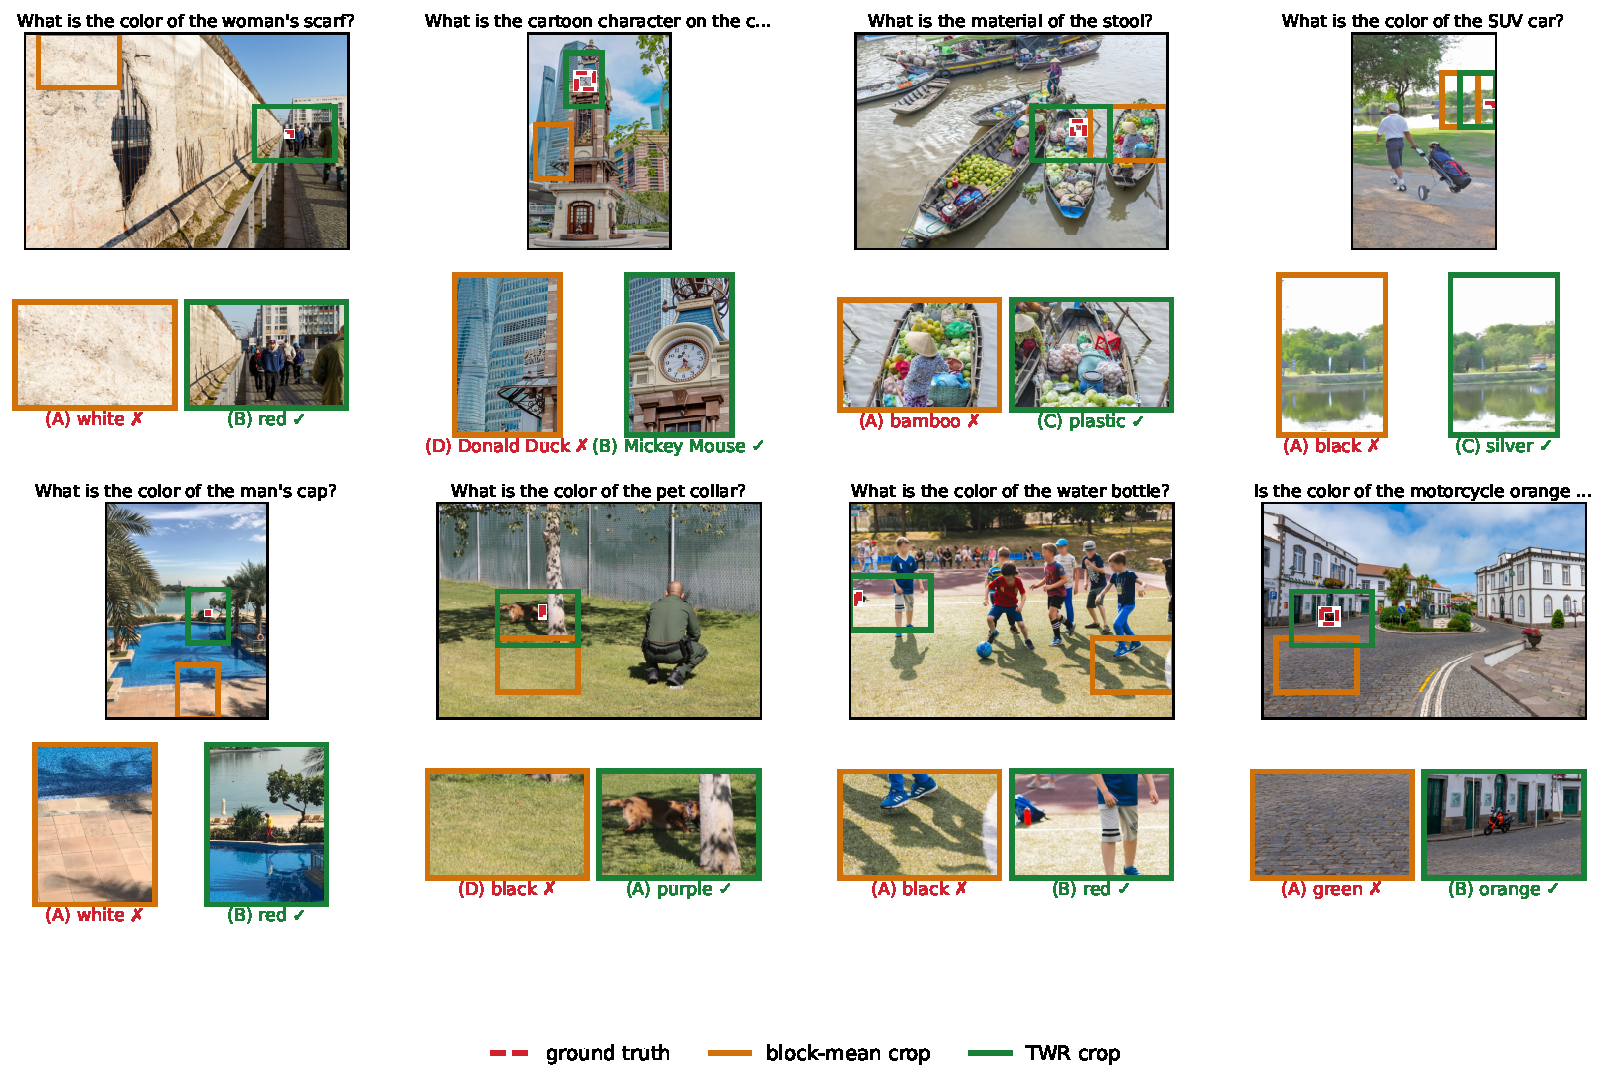
\includegraphics[width=\textwidth]{figs/fig_gallery_twr_q3.pdf}
\caption{\textbf{Eight inferences, Qwen3-VL-2B.} Top of each cell: the image with the ground-truth box, the
block-mean crop and the DWA crop. Below: the two crops the model actually answers from, with its answer.}
\label{fig:galtwr3}
\end{figure}

\begin{figure}[h]\centering
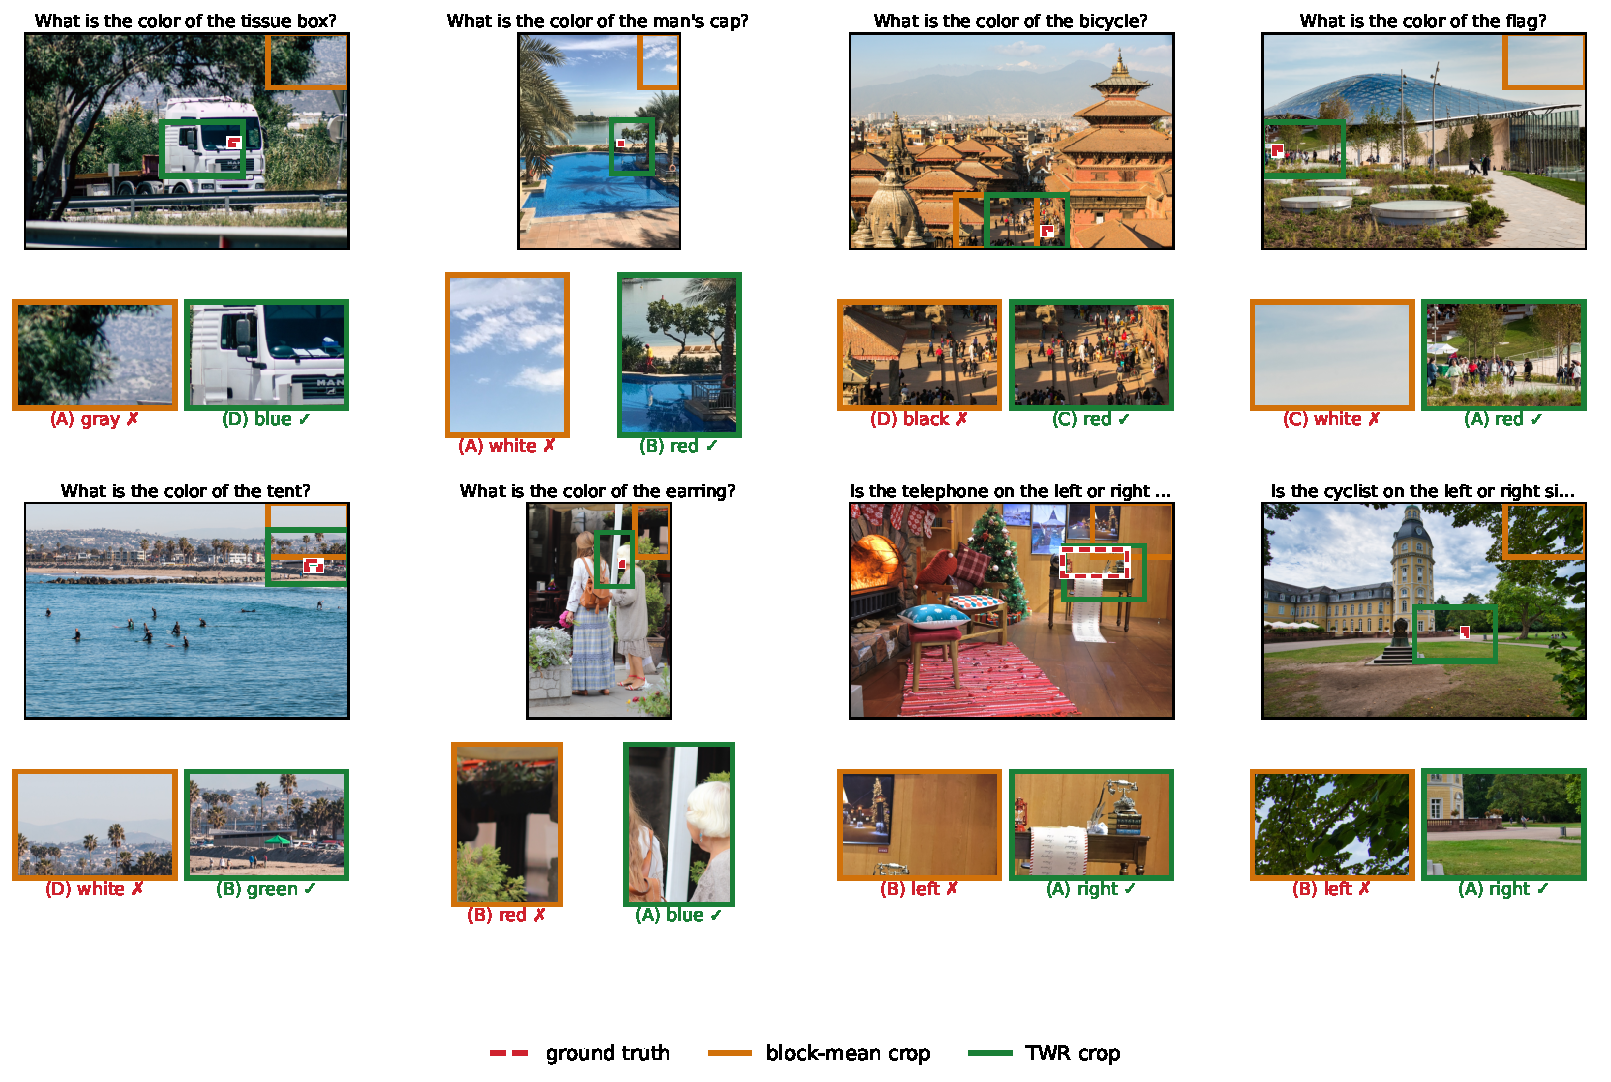
\includegraphics[width=\textwidth]{figs/fig_gallery_twr_q2.pdf}
\caption{\textbf{The same eight-item view on Qwen2-VL-7B.} The failure mode is the same on a different model
family and a different parameter count.}
\label{fig:galtwr2}
\end{figure}

\begin{figure}[h]\centering
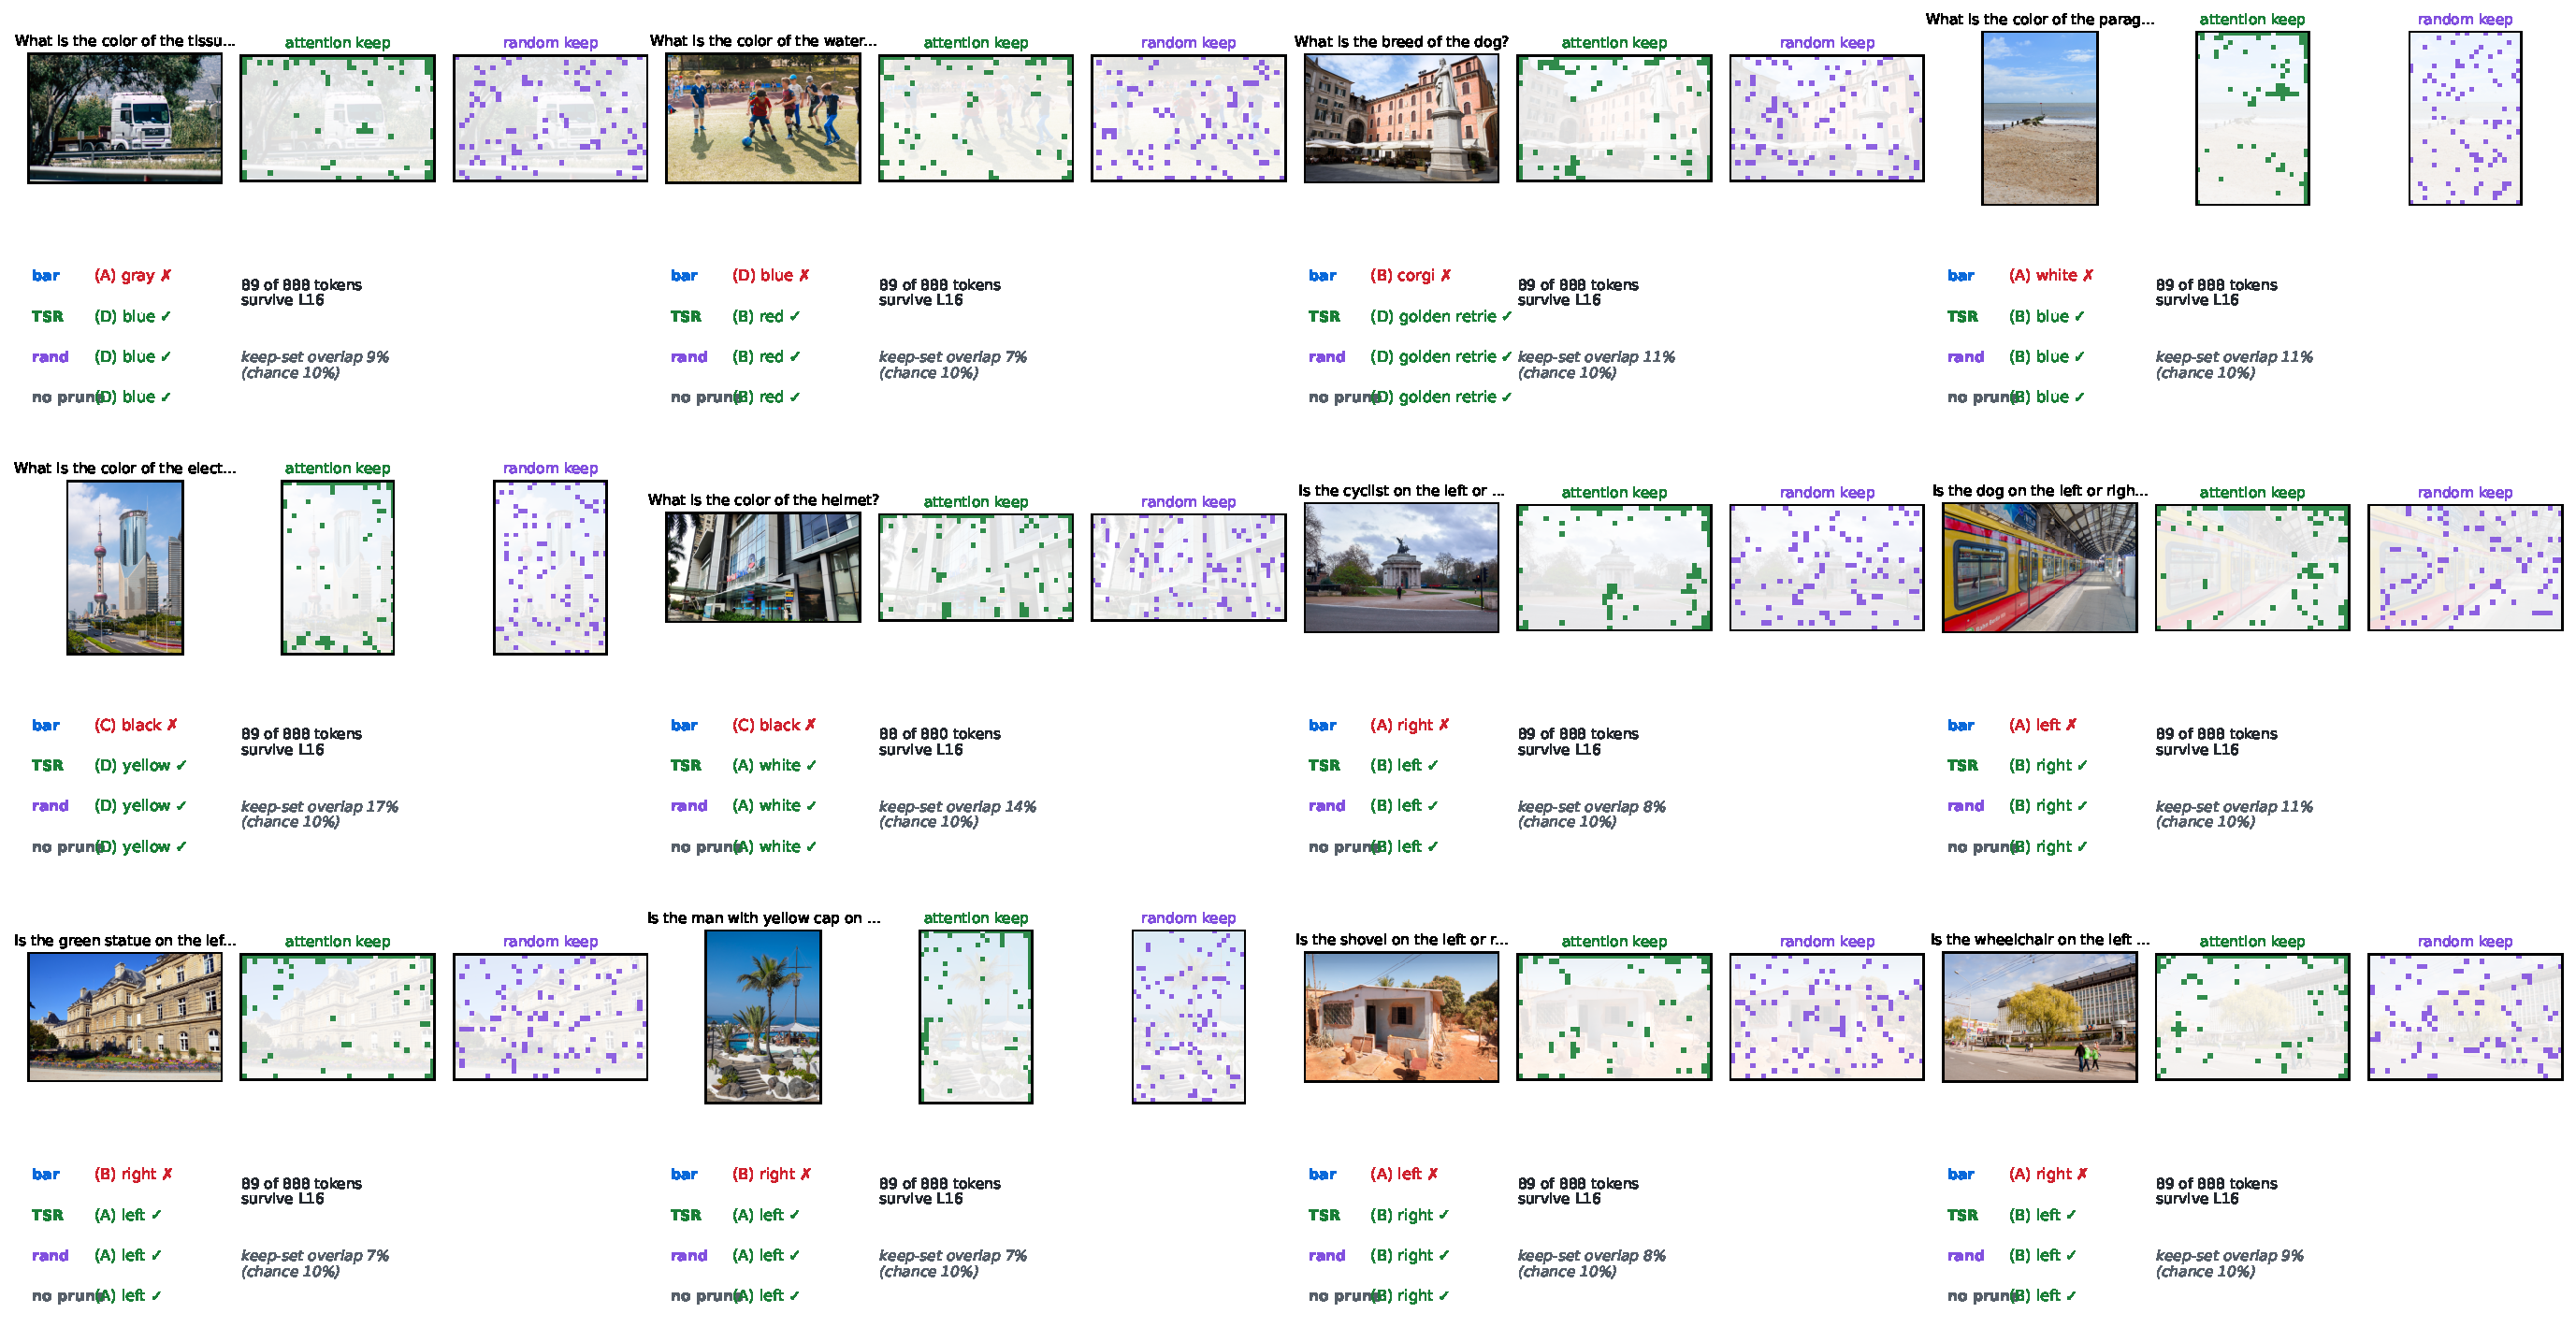
\includegraphics[width=\textwidth]{figs/fig_gallery_tsr.pdf}
\caption{\textbf{Twelve inferences under AVR.} For each item: the image, the tokens kept by attention at the
boundary, and an equally sized random keep. The two keep-sets overlap at close to the $10\%$ chance rate and the
model answers identically under both, and identically again without pruning at all.}
\label{fig:galtsr}
\end{figure}

\begin{figure}[h]\centering
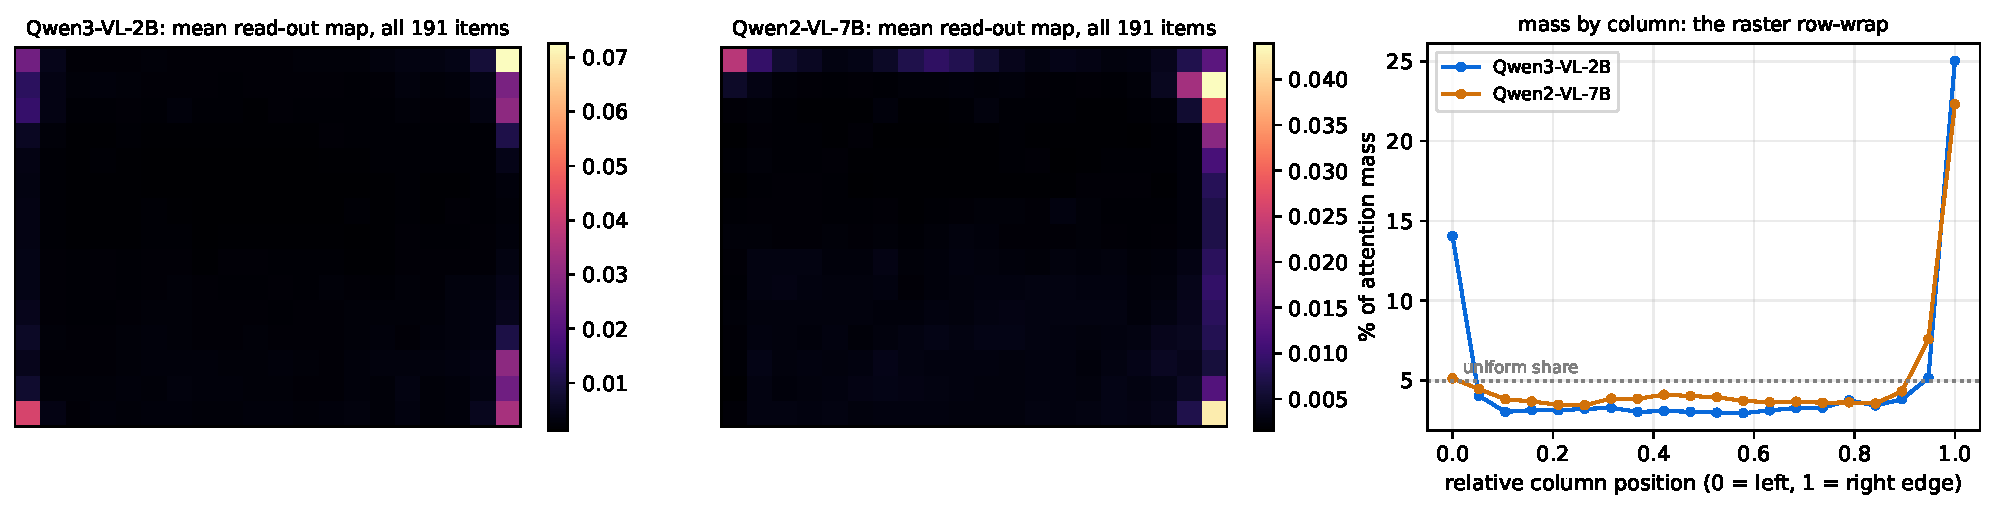
\includegraphics[width=\textwidth]{figs/fig_sink_map.pdf}
\caption{\textbf{The serialisation sink, averaged over the benchmark.} Each item's read-out map is resampled to a
common grid and averaged over all $191$ items. Mass concentrates in the last column --- the token before a raster
row-wrap --- on both checkpoints, at roughly four times the uniform share. This is what the outer-ring mask in
every deployed implementation is patching around.}
\label{fig:sink}
\end{figure}

\begin{figure}[h]\centering
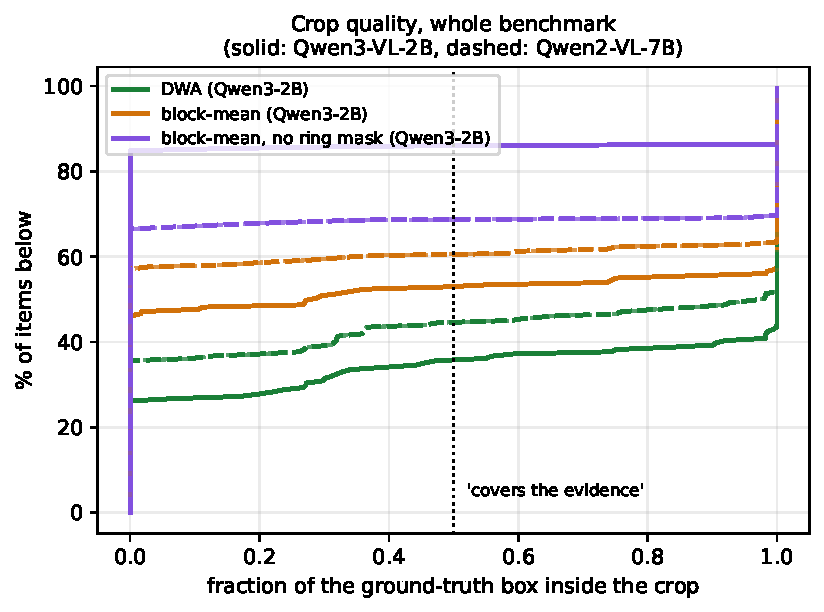
\includegraphics[width=0.56\textwidth]{figs/fig_coverage_cdf.pdf}
\caption{\textbf{Crop quality over the whole benchmark.} Cumulative distribution of the fraction of the
ground-truth box captured by the crop. Without the ring mask the block-mean rule is close to useless; with it,
it is usable; DWA is better than both and barely uses the mask.}
\label{fig:covcdf}
\end{figure}

\section{Method ablations}\label{app:abl}

\textbf{Window size.} $W$ is a first-order hyperparameter, and the right value is set by the same condition that
sets the sign. At an equal answer budget ($300$ vs $300$ tokens, identical items), \vstar\ wants the tight window:
$W{=}0.25$ scores $72.8$ against $W{=}0.5$'s $62.3$ and the full image's $53.9$. On text and documents the
ordering reverses --- the tight window clips words and drops the referent --- and $W{=}0.5$ recovers most of the
gap: TextVQA $49.8 \to 67.9$ and DocVQA $35.2 \to 50.3$ at the same budget, still below the no-crop arms
($74.7$ and $56.0$). A dynamic rule that sizes the window from the ridge score's top-5\% bounding box degenerates
to a wide window (mean $W$ $0.46$--$0.47$; $64$--$71\%$ of items at the $0.50$ clamp) and tracks $W{=}0.5$ rather
than adapting; reported as a negative for that rule, not for dynamism in general.

\textbf{Per-head statistics.} The deployed read-out averages over heads. Adding, per layer, the per-cell maximum
over heads and the head-distribution std ($91$ features instead of $63$) raises out-of-fold coverage from $0.605$
to $0.630$ on Qwen3 and $0.581$ to $0.609$ on Qwen2. End-task the gain is $+1.0$ [$-4.2,+6.3$] on \vstar\ and
$+2.4$ [$-1.0,+5.8$] on TextVQA: positive in both cells, significant in neither. The coverage gain does not
convert --- another instance of the intermediate-metric gap (Appendix~\ref{app:proxy}) --- so the head-augmented
filter is kept as an option rather than as the deployed method.

\section{The map-only policy in full}\label{app:policy}

Policy $-$ equal-compute bar, paired item bootstrap ($8000$ resamples). The gate is the AND of
$\mathrm{disp}$, $\mathrm{band\_disp}$ and $\mathrm{VRH}$ above their item-set medians; the arms are
DWA@$300$ (crop) and AVR (whole image). Strata are only defined on
\vstar\ and HR-4K. Script: \texttt{phase237\_policy\_final.py}.

\begin{table}[h]\centering\small
\caption{\textbf{Full intervals for the map-only policy.}}
\footnotesize\setlength{\tabcolsep}{3pt}
\begin{tabular}{llcccc}
\toprule
model & benchmark & route\% & policy $-$ bar & single & cross\\
\midrule
Qwen3-VL-2B & \vstar & $36$ & $+10.5\,[+4.2,+17.3]$ & $+9.6\,[+0.9,+18.3]$ & $+11.8\,[+3.9,+19.7]$\\
Qwen3-VL-2B & HR-4K & $32$ & $+3.9\,[+1.4,+6.4]$ & $+7.0\,[+3.0,+11.0]$ & $+0.8\,[-2.3,+4.0]$\\
Qwen3-VL-2B & CV-Bench & $35$ & $-3.3\,[-4.6,-2.0]$ & --- & ---\\
Qwen3-VL-2B & RealworldQA & $34$ & $+0.8\,[-1.8,+3.4]$ & --- & ---\\
Qwen2-VL-7B & \vstar & $38$ & $+7.9\,[+1.6,+14.1]$ & $+10.4\,[+2.6,+18.3]$ & $+3.9\,[-5.3,+13.2]$\\
Qwen2-VL-7B & HR-4K & $28$ & $+4.5\,[+1.8,+7.2]$ & $+8.0\,[+4.0,+12.2]$ & $+1.0\,[-2.8,+4.8]$\\
Qwen2-VL-7B & CV-Bench & $28$ & $-3.4\,[-5.0,-1.9]$ & --- & ---\\
Qwen2-VL-7B & RealworldQA & $34$ & $+0.0\,[-6.2,+6.2]$ & --- & ---\\
\bottomrule
\end{tabular}\label{tab:policyfull}
\end{table}

\section{Designs that did not work}\label{app:neg}

\begin{table}[h]\centering\small
\caption{The ten designs intended to extend cropping to cross-instance questions, and the two that tried to
combine the two policies. Each was pre-registered with a primary contrast and a guard before it ran. ``Cleared''
counts checkpoints of two on which the primary passed.}
\begin{tabular}{p{3.2cm}p{3.5cm}cp{4.5cm}}
\toprule
design & what it changed & cleared & diagnosed cause\\
\midrule
per-item window sizer & crop size from map features & 0/2 & grid inversion, weak features\\
peak-spanning window & box spanning the top peaks & 0/2 & relative signal, absolute constant\\
mass-containment window & window holding $x\%$ of mass & 0/2 & boxes far too large\\
joint cell-window ranking & arg-max over both at once & 0/2 & metric artefact: coverage rises with size\\
expected-accuracy window & window by predicted accuracy & 0/2 & accuracy--size curve flat against noise\\
thumbnail in answer pass & crop plus $64$-token scene & 0/2 & second object below the encoding cliff\\
global--local split & scene@150 plus crop@150 & 0/2 & halving the crop costs more than the scene gives\\
context-continued crop & scene@300 plus crop@300 & 0/2 & scene costs $8.7$ and $5.2$ even with a perfect crop\\
multi-crop, matched budget & $2\times150$ and $3\times100$ & 0/2 & magnification tax ($-11.3$, $-4.3$) exceeds coverage gain ($+7.8$, $+2.6$)\\
funded multi-crop & $2\times300$, pruned, early exit & 0/2 & $+3.7$ on one model, $-2.6$ on the other\\
DWA-guided early pruning & rank at L4 instead of L16 & 0/2 & $-5.2$: ranking before transport is worthless\\
AVR stacked on a placement rule & crop@$460$ pruned at L16, same budget & 0/2 & no resolution headroom left on a crop ($+0.8$ vs $+4.5$)\\
\bottomrule
\end{tabular}\label{tab:neg}
\end{table}

The last row generalises the rest, and explains why the two policies cannot be merged into one. DWA's signal
is produced after the transport boundary, and pruning only saves compute at or before it. A pipeline that prunes
early enough to save has destroyed the layers DWA reads, which costs $3.1$ and $12.6$ points of coverage; a
pipeline that waits for DWA has nothing left worth pruning. Holding the ranking fixed and moving only the cut
from L16 to L4 costs $5.2$ points. The incompatibility is structural, not a tuning failure.

\paragraph{The two policies are substitutes, not complements.} The structural argument above is not the only
reason they do not combine. We also tested the composition that \emph{is} mechanically sound: hold the token-layer
budget fixed, and let any placement rule spend its answer pass on a crop encoded at $460$ tokens and pruned $90\%$
at the boundary instead of a plain crop at $300$. Applied to ViCrop-style block-mean, to LASER, to DWA and to
oracle placement, on both checkpoints, every one of the eight contrasts spans zero. The diagnostic says why: the
resolution headroom left \emph{on a crop} averages $+0.8$ points, against $+4.5$ on the full image. A
$0.25\times0.25$ window re-encoded at $300$ tokens has already lifted the object above the encoding cliff, so the
magnification AVR would buy has already been spent. Both policies spend the same resource, effective resolution on
the region that matters; cropping spends it in a targeted way and AVR spends it uniformly. That is why their
\emph{scope} is complementary while their \emph{gains} are not additive.

\paragraph{Why cropping cannot reach cross-instance questions.} Under \emph{perfect} placement, cross-instance
accuracy reaches $75.0$ and $77.6$, an irreducible error of $25\%$ and $22\%$, against $3.5\%$ and $6.1\%$ for
single-instance. Two crops at full resolution covering \emph{both} objects, which raises cross-instance object coverage by
$17.1$ and $15.8$ points, still score $-2.6$ and $-3.9$ against a single crop. Cross-instance error is not predominantly perceptual, so no
reallocation of perceptual resources reaches it. Resolution does reach part of it, which is what the second policy
exploits, but cropping does not.

\section{Pipeline faults found, and how they were caught}\label{app:faults}

Two runs in this work produced plausible numbers that were wrong. We report them because the rules that caught them
are the reason we trust the rest, and because both faults are easy to make and invisible in aggregate accuracy.

\paragraph{A silently unpatched module.} Pruning is injected by monkey-patching the attention forward pass. The
patch covered two module paths; a third checkpoint's attention lived in a third module, so pruning was a no-op and
the arm was byte-identical to its unpruned control while reporting a clean $+12.2$. It was caught by a standing
rule: a contrast of exactly $+0.0$ with a $[+0.0,+0.0]$ interval is a pipeline fault, never a result, because real
effects do not land on zero to machine precision. The fix asserts at load time that the model's actual attention
module is one the patch reached, and prints it every run.

\paragraph{A hard-coded depth on a differently-shaped model.} The arm table hard-coded the prune layer at $16$. On
the $36$-layer checkpoint the correct depth, $0.57\times36=21$, was computed and printed but never used, so the run
pruned at $44\%$ of depth, inside the transport window. It was caught by the compute budget reading $78\%$ of the
bar instead of the expected $98\%$. We retain the voided run as accidental evidence for the boundary itself:
pruning inside the window cost $-7.9$ pooled and $-10.5$ cross-instance on a third model family.

Every arm therefore prints its realised token count and its token-layer budget as a fraction of the bar, and any
run outside $96$--$104\%$ is discarded rather than reported.

